\documentclass[10pt,letterpaper,twocolumn,twosided]{article}

\usepackage[utf8]{inputenc}
\usepackage[spanish]{babel}
\usepackage{listings}
\usepackage[usenames,dvipsnames]{color}
\usepackage{amsmath}
\usepackage{verbatim}
\usepackage{hyperref}
\usepackage{color}
\usepackage{geometry}
\usepackage{multicol}
\usepackage{multirow}
\usepackage{supertabular}
\usepackage{booktabs}
\usepackage{graphicx}
\geometry{verbose,landscape,letterpaper,tmargin=2cm,bmargin=2cm,lmargin=1cm,rmargin=1cm}

\usepackage{listings}
\usepackage{color}

\definecolor{dkgreen}{rgb}{0,0.6,0}
\definecolor{gray}{rgb}{0.5,0.5,0.5}
\definecolor{mauve}{rgb}{0.58,0,0.82}

\lstset{frame=tb,
  language=C++,
  aboveskip=3mm,
  belowskip=3mm,
  showstringspaces=false,
  columns=flexible,
  basicstyle={\small\ttfamily},
  numbers=none,
  numberstyle=\tiny\color{gray},
  keywordstyle=\color{blue},
  commentstyle=\color{dkgreen},
  stringstyle=\color{mauve},
  breaklines=true,
  breakatwhitespace=true
  tabsize=2,
  literate=
  {á}{{\'a}}1 {é}{{\'e}}1 {í}{{\'i}}1 {ó}{{\'o}}1 {ú}{{\'u}}1 {ñ}{{\~n}}1
  {Á}{{\'A}}1 {É}{{\'E}}1 {Í}{{\'I}}1 {Ó}{{\'O}}1 {Ú}{{\'U}}1 {Ñ}{{\~N}}1
  {à}{{\`a}}1 {è}{{\`e}}1 {ì}{{\`i}}1 {ò}{{\`o}}1 {ù}{{\`u}}1
  {À}{{\`A}}1 {È}{{\'E}}1 {Ì}{{\`I}}1 {Ò}{{\`O}}1 {Ù}{{\`U}}1
  {ä}{{\"a}}1 {ë}{{\"e}}1 {ï}{{\"i}}1 {ö}{{\"o}}1 {ü}{{\"u}}1
  {Ä}{{\"A}}1 {Ë}{{\"E}}1 {Ï}{{\"I}}1 {Ö}{{\"O}}1 {Ü}{{\"U}}1
  {â}{{\^a}}1 {ê}{{\^e}}1 {î}{{\^i}}1 {ô}{{\^o}}1 {û}{{\^u}}1
  {Â}{{\^A}}1 {Ê}{{\^E}}1 {Î}{{\^I}}1 {Ô}{{\^O}}1 {Û}{{\^U}}1
  {œ}{{\oe}}1 {Œ}{{\OE}}1 {æ}{{\ae}}1 {Æ}{{\AE}}1 {ß}{{\ss}}1
  {ű}{{\H{u}}}1 {Ű}{{\H{U}}}1 {ő}{{\H{o}}}1 {Ő}{{\H{O}}}1
  {ç}{{\c c}}1 {Ç}{{\c C}}1 {ø}{{\o}}1 {å}{{\r a}}1 {Å}{{\r A}}1
  {€}{{\EUR}}1 {£}{{\pounds}}1
}

\setlength{\columnsep}{0.5in}
\setlength{\columnseprule}{1px}

\begin{document}

\title{ICPC Notebook - UNAL}
\author{Universidad Nacional de colombia}
\maketitle
\tableofcontents
\lstloadlanguages{Java}

% MISCELLANEOUS
\section{Miscellaneous}

\subsection{Miscellaneous}
\begin{lstlisting}
#define between(a, b, c) (a <= b && b <= c)
#define has_key(it, key) (it.find(key) != it.end())
#define check_coord(x, y, n, m) (0 <=x && x < n && 0 <= y && y < m)

const int d4x[4] = {0, -1, 1, 0};
const int d4y[4] = {-1, 0, 0, 1};
const int d8x[8] = {-1, 0, -1, 1, -1, 1, 0, 1};
const int d8y[8] = {-1, -1, 0, -1, 1, 0, 1, 1};

#define endl '\n'
#define _ << ' ' <<
#define PB push_back
#define SZ(v) ((int) v.size())
#define trav(ref, ds) for(auto &ref: ds)
#define forn(i, b) for(int i = 0; i < int(b); ++i)
#define forr(i, b) for(int i = int(b)-1; i >= 0; i--)
#define rep(i, a, b) for(int i = int(a); i <= int(b); ++i)
#define rev(i, b, a) for(int i = int(b); i >= int(a); i--)

#define precise(n,k) fixed << setprecision(k) << n

#define all(x) (x).begin(), (x).end()
#define rall(x) (x).rbegin(), (x).rend()
#define ms(arr, value) memset(arr, value, sizeof(arr))

template<typename T>
inline void unique(vector<T> &v) {
    sort(v.begin(), v.end());
    v.resize(distance(v.begin(), unique(v.begin(), v.end())));
}

#define infinity while(1)
#define unreachable assert(false && "Unreachable");

#pragma GCC optimize("O3,unroll-loops")
#pragma GCC target("avx2,bmi,bmi2,lzcnt,popcnt")

// THINGS TO KEEP IN MIND
//   * int overflow, time and memory limits
//   * Special case (n = 1?)
//   * Do something instead of nothing and stay organized
//   * Don't get stuck in one approach
 
// TIME AND MEMORY LIMITS
//   * 1 second is approximately 10^8 operations (c++)
//   * 10^6 Elements of 32 Bit (4 bytes) is equal to 4 MB
//   * 62x10^6 Elements of 32 Bit (4 bytes) is equal to 250 MB
//   * 10^6 Elements of 64 Bits (8 bytes) is equal to 8 MB
//   * 31x10^6 Elements of 64 Bit (8 bytes) is equal to 250 MB

ios::sync_with_stdio(0);
cin.tie(0);

// Lectura segun el tipo de dato (Se usan las mismas para imprimir):

scanf("%d", &value); //int
scanf("%ld", &value); //long y long int
scanf("%c", &value); //char 
scanf("%f", &value); //float
scanf("%lf", &value); //double
scanf("%s", &value); //char*
scanf("%lld", &value); //long long int
scanf("%x", &value); //int hexadecimal
scanf("%o", &value); //int octal

// Impresion de punto flotante con d decimales, ejemplo 6 decimales:
printf("%.6lf", value);

// Genera un numero entero aleatorio en el rango [a, b]. Para ll usar "mt19937_64" y cambiar todo a ll.

mt19937 rng(chrono::steady_clock::now().time_since_epoch().count());
int rand(int a, int b) {
    return uniform_int_distribution<int>(a, b)(rng);
}

vector<string> split(string str, string separator) {
    vector<string> tokens;
    for ( auto tok = strtok(&str[0], separator.data());
            tok != NULL;
            tok = strtok(NULL, separator.data())) {
        tokens.push_back(tok);
    }
    return tokens;
}

// Custom hashing for secure unordered_map
struct custom_hash {
    size_t operator()(uint64_t x) const {
        static const uint64_t FIXED_RANDOM = 
            chrono::steady_clock::now().time_since_epoch().count();
        x ^= FIXED_RANDOM;
        return x ^ (x >> 16);
    }
};

unordered_map<ll, int, custom_hash> safe_map;
gp_hash_table<ll, int, custom_hash> safe_hash_table;
safe_map.reserve(1024); // Power of 2
safe_map.max_load_factor(0.25);

// Python Read
from sys import stdin, stdout
list(map(func, stdin.readline().strip().split()))
\end{lstlisting}

\subsection{Stress Testing Script}
\begin{lstlisting}
# A and B are executables you want to compare, gen takes int
# as command line arg. Usage: 'sh stress.sh'
for ((i = 1; ; ++i)); do  # if they are same then will loop forever
    echo $i
    ./gen $i > int
    ./A < int > out1
    ./B < int > out2
    diff -w out1 out2 || break
    # diff -w <(./A < int) <(./B < int) || break
done
\end{lstlisting}

% STD LIBRARY

\section{STD Library}

\subsection{Find Nearest Set}
\begin{lstlisting}
// Finds the element nearest to target
template<typename T>
T find_nearest(set<T> &st, T target) {
    assert(!st.empty());
    auto it = st.lower_bound(target);
    if (it == st.begin()) {
        return *it;
    } else if (it == st.end()) {
        it--; return *it;
    }
    T right = *it; it--;
    T left = *it;
    if (target-left < right-target) 
        return left;
    // if they are the same distance, choose right
    // if you want to choose left change to <=
    return right;
}
\end{lstlisting}


\subsection{Merge Vector}
\begin{lstlisting}
template<typename T> // To merge two vectors, the answer is an ordered vector
void merge_vector(vector<T> &big, vector<T> &small) {
    int n = (int) big.size();
    int m = (int) small.size();
    if(m > n) swap(small, big);
    if(!is_sorted(big.begin(), big.end()))
        sort(big.begin(), big.end());
    if(!is_sorted(small.begin(), small.end()))
        sort(small.begin(), small.end());
    vector<T> aux;
    merge(small.begin(), small.end(), big.begin(), big.end(), aux.begin());
    big = move(aux);
}
\end{lstlisting}

\subsection{Shorter - Priority Queue}
\begin{lstlisting}
template<typename T, typename Sequence=vector<T>, typename Compare=less<T>>
using template_heap = priority_queue<T, Sequence, Compare>;

template<typename T>
using max_heap = template_heap<T>;

template<typename T>
using min_heap = template_heap<T, vector<T>, greater<T>>;

#define pop_heap(heap) heap.top(); heap.pop();
\end{lstlisting}

\subsection{Rope}
\begin{lstlisting}
#include <ext/rope>
using namespace __gnu_cxx;
#define trav_rope(it, v) for(auto it=v.mutable_begin(); it!= v.mutable_end(); ++it)
#define all_rope(rp) (rp).mutable_begin(), (rp).mutable_end()
// trav_rope(it, v) cout << *it << " ";
// Use `crope` for strings
// push_back(T val): 
//      This function is used to input a character at the end of the rope
//      Time Complexity: O(log2(n))
// pop_back():
//      this function is used to delete the last character from the rope
//      Time Complexity: O(log2(n))
// insert(int i, rope r): !!!!!!!!!!!!!!!!WARING!!!!!!!!!!! Worst Case: O(N).
//      Inserts the contents of `r` before the i-th element.
//      Time Complexity: Best Case: O(log N) and Worst Case: O(N). 
// erase(int i, int n):
//      Erases n elements, starting with the i-th element
//      Time Complexity: O(log2(n))
// substr(int i, int n):
//      Returns a new rope whose elements are the n elements starting at the position i-th
//      Time Complexity: O(log2(n))
// replace(int i, int n, rope r):
//      Replaces the n elements beginning with the i-th element with the elements in r
//      Time Complexity: O(log2(n))
// concatenate(+):
//      Concatenate two ropes using the ‘+’ symbol
//      Time Complexity: O(1)
\end{lstlisting}

\subsection{Set Utilities}
\begin{lstlisting}
template<typename T>
T get_min(set<T> &st) {
    assert(!st.empty());
    return *st.begin();
}
template<typename T>
T get_max(set<T> &st) {
    assert(!st.empty());
    return *st.rbegin();
}
template<typename T>
T erase_min(set<T> &st) {
    assert(!st.empty());
    T to_return = get_min(st);
    st.erase(st.begin());
    return to_return;
}
template<typename T>
T erase_max(set<T> &st) {
    assert(!st.empty());
    T to_return = get_max(st);
    st.erase(--st.end());
    return to_return;
}
#define merge_set(big, small) big.insert(small.begin(), small.end());
#define has_key(it, key) (it.find(key) != it.end())
\end{lstlisting}

\subsection{To Reverse Utilities}
\begin{lstlisting}
template<typename T>
class to_reverse {
private:
    T& iterable_;
public:
    explicit to_reverse(T& iterable) : iterable_{iterable} {}
    auto begin() const { return rbegin(iterable_); }
    auto end() const { return rend(iterable_); }
};
\end{lstlisting}

% DATA STRUCTURE

\section{Data Structure}

\subsection{Disjoint Set Union}
\begin{lstlisting}
struct DSU {
    vector<int> par, sizes;
    int size;
    DSU(int n) : par(n), sizes(n, 1) {
        size = n;
        iota(par.begin(), par.end(), 0);
    }
    // Busca el nodo representativo del conjunto de u
    int find(int u) {
        return par[u] == u ? u : (par[u] = find(par[u]));
    }
    // Une los conjuntos de u y v
    void unite(int u, int v) {
        u = find(u), v = find(v);
        if (u == v) return;
        if (sizes[u] > sizes[v]) swap(u,v);
        par[u] = v;
        sizes[v] += sizes[u];
        size--;
    }
    // Retorna la cantidad de elementos del conjunto de u
    int count(int u) { return sizes[find(u)]; }
};
\end{lstlisting}

\subsection{Min - Max Queue}
\begin{lstlisting}
// Permite hallar el elemento minimo para todos los subarreglos de un largo fijo en O(n). Para Max queue cambiar el > por <.
struct min_queue {
    deque<int> dq, mn;
    void push(int x) {
        dq.push_back(x);
        while (mn.size() && mn.back() > x) mn.pop_back();
        mn.push_back(x);
    }
    void pop() {
        if (dq.front() == mn.front()) mn.pop_front();
        dq.pop_front();
    }
    int min() { return mn.front(); }
};
\end{lstlisting}

\vfill

\subsection{Prefix Sum Immutable 2D}
\begin{lstlisting}
template<typename T>
class PrefixSum2D {
public:
    int n, m;
    vector<vector<T>> dp;

    PrefixSum2D()  : n(-1), m(-1) {}
    PrefixSum2D(vector<vector<T>>& grid) {
        n = (int) grid.size();
        assert(0 <= n);
        if(n == 0) { m = 0; return; }
        m = (int) grid[0].size();
        dp.resize(n+1, vector<T>(m+1, static_cast<T>(0)));
        
        for(int i = 1; i <= n; ++i)
            for(int j = 1; j <= m; ++j)
                dp[i][j] = dp[i][j-1] + grid[i-1][j-1];
        for(int j = 1; j <= m; ++j)
            for(int i = 1; i <= n; ++i)
                dp[i][j] += dp[i-1][j];
    }
    T query(int x1, int y1, int x2, int y2) {
        assert(0<=x1&&x1<n && 0<=y1&&y1<m);
        assert(0<=x2&&x2<n && 0<=y2&&y2<m);
        int SA = dp[x2+1][y2+1];
        int SB = dp[x1][y2+1];
        int SC = dp[x2+1][y1];
        int SD = dp[x1][y1];
        return SA-SB-SC+SD;
    }
};

// Prefix Sum Immutable 2D - Shorter code
const int N = 102;
const int M = 102;
const int inf = 1e9;

int n;
int a[N][M];
int sum[N][M];

int query(int x1, int z1, int x2, int z2){
    return sum[x2][z2] + sum[x1-1][z1-1] - sum[x1-1][z2] - sum[x2][z1-1];
}

// initialization / at main()

for(int i = 1; i <= n; ++i) {
    for(int j = 1; j <= m; ++j) {
        cin >> a[i-1][j-1]; // 0-Indexed
        sum[i][j] = sum[i-1][j] + sum[i][j-1] - sum[i-1][j-1] + a[i-1][j-1];
    }
}

// query(x1, z1, x2, z2)
\end{lstlisting}

\subsection{Prefix Sum}
\begin{lstlisting}
template<typename T>
class PrefixSum {
public:
    int n;
    vector<T> dp;
    PrefixSum() : n(-1) {}
    PrefixSum(vector<T>& nums) {
        n = (int) nums.size();
        if(n == 0)
            return;
        dp.resize(n + 1);
        dp[0] = 0;
        for(int i = 1; i <= n; ++i)
            dp[i] = dp[i-1] + nums[i-1];
    }
    T query(int left, int right) {
        assert(0 <= left && left <= right && right <= n - 1);
        return dp[right+1] - dp[left];
    }
};
\end{lstlisting}

\subsection{Segment Tree Lazy}
\begin{lstlisting}
using int64 = long long;
const int64 nil = 1e18; // for sum: 0, for min: 1e18, for max: -1e18
int64 op(int64 x, int64 y) { return min(x, y); }

struct segtree_lazy {
    segtree_lazy *left, *right;
    int l, r, m;
    int64 sum, lazy;

    segtree_lazy(int l, int r) : l(l), r(r), sum(nil), lazy(0) {
        if(l != r) {
            m = (l+r)/2;
            left = new segtree_lazy(l, m);
            right = new segtree_lazy(m+1, r);
        }
    }
    /// (l, l+1, l+2 .... r-1, r)
    /// x   x     x     x  x x x 
    /// (cuantos tengo) * x
    /// r-l+1
    void propagate() {
        if(lazy != 0) {
            /// voy a actualizar el nodo
            sum += (r - l + 1) * lazy;
            if(l != r) {
                left->lazy += lazy;
                right->lazy += lazy;
            }
            /// voy a propagar a mis hijos
            lazy = 0;
        }
    }
    // void modify(int pos, int v) {
    //     if(l == r) {
    //         sum = v;
    //     } else {
    //         if(pos <= m) left->modify(pos, v);
    //         else right->modify(pos, v);
    //         sum = op(left->sum, right->sum);
    //     }
    // }
    void modify(int a, int b, int64 v) {
        propagate();
        if(a > r || b < l) return;
        if(a <= l && r <= b) {
            lazy = v; // lazy += v, for add
            propagate();
            return;
        }
        left->modify(a, b, v);
        right->modify(a, b, v);
        sum = op(left->sum, right->sum);
    }

    int64 query(int a, int b) {
        propagate();
        if(a > r || b < l) return nil;
        if(a <= l && r <= b) return sum;
        return op(left->query(a, b), right->query(a, b));
    }
};
\end{lstlisting}

\subsection{Segment Tree Standard}
\begin{lstlisting}
// Reference: descomUNAL's Notebook
using int64 = long long;
const int64 nil = 1e18; // for sum: 0, for min: 1e18, for max: -1e18
int64 op(int64 x, int64 y) { return min(x, y); }
struct segtree {
    segtree *left, *right;
    int l, r, m;
    int64 sum;
    segtree(int l, int r) : l(l), r(r), sum(nil) {
        if(l != r) {
            m = (l+r)/2;
            left = new segtree(l, m);
            right = new segtree(m+1, r);
        }
    }
    void modify(int pos, int64 v) {
        if(l == r) {
            sum = v;
        } else {
            if(pos <= m) left->modify(pos, v);
            else right->modify(pos, v);
            sum = op(left->sum, right->sum);
        }
    }
    int64 query(int a, int b) {
        if(a > r || b < l) return nil;
        if(a <= l && r <= b) return sum;
        return op(left->query(a, b), right->query(a, b));
    }
};
// Usage:
// segtree st(0, n);
// forn(i, n) {
//    cin >> val;
//    st.modify(i, val);
// }
\end{lstlisting}

\subsection{Sparse Table}
\begin{lstlisting}
struct RMQ {
    vector<vector<int>> table;
    RMQ(vector<int> &v) : table(20, vector<int>(v.size())) {
        int n = v.size();
        for (int i = 0; i < n; i++)
            table[0][i] = v[i];
        for (int j = 1; (1<<j) <= n; j++)
            for (int i = 0; i + (1<<(j-1)) < n; i++)
                table[j][i] = min(table[j-1][i], table[j-1][i + (1<<(j-1))]);
    }
    int query(int a, int b) {
        int j = 31 - __builtin_clz(b-a+1);
        return min(table[j][a], table[j][b-(1<<j)+1]);
    }
};
\end{lstlisting}

\subsection{Tree Order Statistic}
\begin{lstlisting}
#include <bits/stdc++.h>
#include <ext/pb_ds/assoc_container.hpp> 
#include <ext/pb_ds/tree_policy.hpp>

using namespace std;
using namespace __gnu_pbds;

template <typename K, typename V, typename Comp = less<K>>
using indexed_map = tree<K, V, Comp, rb_tree_tag, tree_order_statistics_node_update>;

template <typename K, typename Comp = less<K>>
using indexed_set = indexed_map<K, null_type, Comp>;
// Usage
//    auto it = any.find_by_order(idx); (0-indexed)
//    (*it).first, (*it).second
//    int index = any.order_of_key(key);
//    {1: 10, 2 :20,  5: 50}, order_of_key(3) -> return index 2
\end{lstlisting}

% GRAPH
\section{Graph}

\subsection{Articulation Points}
\begin{lstlisting}
// Encontrar los nodos que al quitarlos, se deconecta el grafo

vector<vector<int>> adj;
vector<bool> visited;
vector<int> low;
// Order in which it was visited
vector<int> order;
vector<bool> points;
// Count the components
int counter = 0;
// Number of Vertex
int vertex;

void dfs(int node, int parent = -1) {
    visited[node] = true;
    low[node] = order[node] = ++counter;

    int children = 0;

    for(int &neighbour: adj[node]) {

        if(!visited[neighbour]) {
            children++;

            dfs(neighbour, node);

            low[node] = min(low[node], low[neighbour]);
            
            // Conditions #1
            if(parent != -1 && order[node] <= low[neighbour]) {
                points[node] = true;
            }
        } else {
            low[node] = min(low[node], order[neighbour]);
        }
    }
    
    // Conditions #2
    if(parent == -1 && children > 1) {
        points[node] = true;
    }
}

vector<int> build() {
    for(int node = 0; node < vertex; ++node)
        if(!visited[node]) dfs(node);
    
    vector<int> output;
    for(int node = 0; node < vertex; ++node)
        if(points[node]) output.push_back(node);
    return output;
}
\end{lstlisting}

\subsection{Bellman Ford}
\begin{lstlisting}
struct edge {
    int from, to;
    int64 cost;
};

int n, m;
const int N = 2505;
const int64 inf = 1e18;
vector<edge> edges;

vector<int64> bellman_ford(int u, bool &cycle) {
    vector<int64> dist(n, inf);
    dist[u] = 0LL;
    for(int i = 0; i < n + 1; ++i){
        for(const edge &e: edges) {
            if(dist[e.from] != inf && dist[e.from] + e.cost < dist[e.to]) {
                dist[e.to] = dist[e.from] + e.cost;
                if(i == n)
                    cycle = true; // There are negative edges
            }
        }
    }
    return dist;
    // Time Complexity: O(V*E), Space Complexity: O(V)
}

// cin >> l >> r >> cost, --l, --r;
// edges.push_back({l, r, cost});
// bool cycle = false;
// vector<int64> dist = bellman_ford(0, cycle);
\end{lstlisting}

\subsection{BFS}
\begin{lstlisting}
// Busqueda en anchura sobre grafos. Recibe un nodo inicial u y visita todos los nodos alcanzables desde u.
// BFS tambien halla la distancia mas corta entre el nodo inicial u y los demas nodos si todas las aristas tienen peso 1.

const int mxN = 1e5+5; // Cantidad maxima de nodos
vector<int> adj[mxN]; // Lista de adyacencia
vector<int64> dist; // Almacena la distancia a cada nodo
int n, m; // Cantidad de nodos y aristas

void bfs(int u) {
    queue<int> Q;
    Q.push(u);
    dist[u] = 0;

    while (Q.size() > 0) {
        u = Q.front();
        Q.pop();
        for (auto &v : adj[u]) {
            if (dist[v] == -1) {
                dist[v] = dist[u] + 1;
                Q.push(v);
            }
        }
    }
}

void init() {
    dist.assign(n, -1);
    for (int i = 0; i <= n; i++) {
        adj[i].clear();
    }
}
\end{lstlisting}


\subsection{Binary Lifting}
\begin{lstlisting}
const int mxN = 2e5 + 10;
const int LOG = 20;

vector<int> adj[mxN];
int up[mxN][LOG];
int tin[mxN];
int tout[mxN];
int depth[mxN];
int timer = 0;

void lifting(int node, int parent) {
    tin[node] = ++timer;
    up[node][0] = parent;
    for(int i = 1; i < LOG; ++i) {
        up[node][i] = up[ up[node][i-1] ][i-1];
        // up[node][i] = up[max(0, up[node][i-1])][i-1]; // to use the jump(node, k) function
    }
    for(auto &child: adj[node]) {
        if(child == parent) continue;
        depth[child] = depth[node] + 1;
        lifting(child, node);
    }
    tout[node] = ++timer;
}

bool is_ancestor(int left, int right) {
    return tin[left] <= tin[right] && tout[left] >= tout[right];
}

int lca(int left, int right) {
    if(is_ancestor(left, right)) {
        return left;
    } else if(is_ancestor(right, left)) {
        return right;
    }
    for(int i = LOG-1; i >= 0; i--) {
        if(!is_ancestor(up[left][i], right)) {
            left = up[left][i];
        }
    }
    return up[left][0];
}

// jump k levels up in the tree
int jump(int node, int k) {
    for(int i = 0; i < LOG; ++i) {
        if((k >> i) & 1 && node != -1) {
            node = up[node][i];
        }
    }
    return node;
}

// distance between 2 nodes -> O(lg(n))
// depth[left] + depth[right] − 2*depth[ lca(left, right) ]

// lifting(0, -1); to use the jump(node, k) function
// lifting(0, 0); to use the lca(left, right) function
\end{lstlisting}

\subsection{Bridges}
\begin{lstlisting}
// Encontrar las aristas que al quitarlas, el grafo queda desconectado

vector<vector<int>> adj;
vector<bool> visited;
vector<int> low;
// Order in which it was visited
vector<int> order;
// Answer:
vector<pair<int, int>> bridges;
// Number of Vertex
int vertex;
// Count the components
int cnt;

void dfs(int node, int parent = -1) {
    visited[node] = true;
    order[node] = low[node] = ++cnt; 
    for (int neighbour: adj[node]) { 
        if (!visited[neighbour]) { 
            dfs(neighbour, node); 
            low[node] = min(low[node], low[neighbour]);

            if (order[node] < low[neighbour]) {
                bridges.push_back({node, neighbour});
            }
        } else if (neighbour != parent)  {
            low[node] = min(low[node], order[neighbour]); 
        }
    }
}

vector<pair<int, int>> build() {
    cnt = 0;
    for (int node = 0; node < adj.size(); node++)
        if (!visited[node]) dfs(node);
    return bridges;
}
\end{lstlisting}

\subsection{Dijkstra}
\begin{lstlisting}
// Dado un grafo con pesos no negativos halla la ruta de costo minimo entre un nodo inicial u y todos los demas nodos.

struct edge {
    int v; int64 cost;
    bool operator < (const edge &other) const {
        return other.cost < cost;
    }
};

const int64 inf = 1e18;
const int N = 1e5+5; // Cantidad maxima de nodos
vector<edge> adj[N]; // Lista de adyacencia
bool was[N];         // Marca los nodos ya visitados
int64 dist[N];       // Almacena la distancia a cada nodo
int pre[N];          // Almacena el nodo anterior para construir las rutas
int n, m;            // Cantidad de nodos y aristas

void dijkstra(int u) {
    priority_queue<edge> Q;
    Q.push({u, 0});
    dist[u] = 0;
    
    while (!Q.empty()) {
        u = Q.top().v; Q.pop();
        if (!was[u]) {
            was[u] = true;
            for (auto &ed : adj[u]) {
                int v = ed.v;
                if (!was[v] && dist[v] > dist[u] + ed.cost) {
                    dist[v] = dist[u] + ed.cost;
                    pre[v] = u;
                    Q.push({v, dist[v]});
                }
            }
        }
    }
}

void init() {
    for (int i = 0; i <= n; i++) {
        adj[i].clear();
        was[i] = 0;
        dist[i] = inf;
    }
}
\end{lstlisting}

\subsection{Floyd Warshall}
\begin{lstlisting}
const int mxN = 500 + 10;
const int64 inf = 1e18;
int64 dp[mxN][mxN];

for(int i = 0; i < n; ++i)
    for(int j = 0; j < n; ++j)
        dp[i][j] = (i == j)? 0 : inf;

// Adding edges
// dp[from][to] = min(dp[from][to], cost);
// dp[to][from] = min(dp[to][from], cost);

for(int k = 0; k < n; ++k) {
    for(int i = 0; i < n; ++i) {
        for(int j = 0; j < n; ++j) {
            if(dp[i][k] < inf && dp[k][j] < inf) {
                dp[i][j] = min(dp[i][j], dp[i][k] + dp[k][j]);
            }
        }
    }
}
// answer: dp[from][to]
\end{lstlisting}

\subsection{Merge Trick on Trees}
\begin{lstlisting}
// Reference: https://usaco.guide/plat/merging?lang=cpp
const int mxN = 2e5 + 10;
vector<int> adj[mxN];
int colors[mxN];
set<int> cnt[mxN];
int answer[mxN];
 
void dfs(int node, int parent) { // O(n*lg^2(n))
    cnt[node].insert(colors[node]);
 
    for(auto &child: adj[node]) {
        if(child == parent) continue;

        dfs(child, node);

        // always make the child set the smallest
        if(cnt[child].size() > cnt[node].size())
            swap(cnt[child], cnt[node]); // O(1)

        // Merge
        for(auto &it: cnt[child]) {
            cnt[node].insert(it);
        }
        cnt[child].clear(); // if time is too high don't use, only use when giving MLE
    }
    answer[node] = (int) cnt[node].size();
}
// dfs(0, -1)
\end{lstlisting}

\subsection{Kahn Algoritm}
\begin{lstlisting}

\end{lstlisting}

\subsection{SCC - Kasaraju}
\begin{lstlisting}
vector<vector<int>> adj;
vector<vector<int>> radj;
vector<bool> visited;
stack<int> toposort;
vector<vector<int>> components; // Answer - SCC
int vertex; // Number of Vertex

// First
// Topological Sort
void toposort_dfs(int node) {
    visited[node] = true;
    for(int neighbour: adj[node]) {
        if(!visited[neighbour]) {
            toposort_dfs(neighbour);
        }
    }
    toposort.push(node);
}

// Second
// dfs Standard - Reverse Adj
void dfs(int node) {
    visited[node] = true;
    components.back().push_back(node);
    for(int neighbour: radj[node]) {
        if(!visited[neighbour]) {
            dfs(neighbour);
        }
    }
}

// Third
// Build Algorithm
vector<vector<int>> build() {
    // Topological Sort
    for(int node = 0; node < vertex; ++node)
        if(!visited[node]) toposort_dfs(node);

    // Reset - Visited
    fill(visited.begin(), visited.end(), false);

    // In the topological order run the reverse dfs
    while(!toposort.empty()) {
        int node = toposort.top();
        toposort.pop();
        if(!visited[node]) {
            components.push_back(vector<int>{});
            dfs(node);
        }
    }
    return components;
}
\end{lstlisting}

\subsection{SCC - Tarjan}
\begin{lstlisting}
// Dado un grafo dirigido halla las componentes fuertemente conexas (SCC).

const int inf = 1e9;
const int MX = 1e5+5; // Cantidad maxima de nodos
vector<int> g[MX]; // Lista de adyacencia
stack<int> st;
int low[MX], pre[MX], cnt;
int comp[MX]; // Almacena la componente a la que pertenece cada nodo
int SCC; // Cantidad de componentes fuertemente conexas
int n, m; // Cantidad de nodos y aristas

void tarjan(int u) {
    low[u] = pre[u] = cnt++;
    st.push(u);
    for (auto &v : g[u]) {
        if (pre[v] == -1) tarjan(v);
        low[u] = min(low[u], low[v]);
    }
    if (low[u] == pre[u]) {
        while (true) {
            int v = st.top(); st.pop();
            low[v] = inf;
            comp[v] = SCC;
            if (u == v) break;
        }
        SCC++;
    }
}

void init() {
    cnt = SCC = 0;
    for (int i = 0; i <= n; i++) {
        g[i].clear();
        pre[i] = -1; // no visitado
    }
}
\end{lstlisting}

\subsection{Topological Sort}
\begin{lstlisting}
class KahnTopoSort {
    vector<vector<int>> adj;
    vector<int> indegree;
    vector<int> toposort;
    int nodes;
    bool solved;
    bool isCyclic;
public:
    
    KahnTopoSort(int n) : nodes(n) {
        adj.resize(n);
        indegree.resize(n, 0);
        solved = false;
        isCyclic = false;
    }
    
    void addEdge(int from, int to) {
        adj[from].push_back(to);
        indegree[to]++;
        solved = false;
        isCyclic = false;
    }
    
    vector<int> sort() {
        if(solved) return toposort;
        toposort.clear();
        queue<int> Q;
        vector<int> in_degree(indegree.begin(), indegree.end());
        for(int i = 0; i < nodes; ++i) {
            if(in_degree[i] == 0) Q.push(i);
        }
        int count = 0;
        while(!Q.empty()) {
            int node = Q.front(); Q.pop();
            toposort.push_back(node);
            for(int neighbour: adj[node]) {
                in_degree[neighbour]--;
                if(in_degree[neighbour] == 0) {
                    Q.push(neighbour);
                }
            }
            count++;
        }
        solved = true;
        if(count != nodes) {
            // There exists a cycle in the graph
            isCyclic = true;
            return vector<int> {};
        }
        return toposort;
    }

    bool getIsCyclic() {
        sort();
        return isCyclic;
    }
};
\end{lstlisting}

\subsection{Topological Sort - Dfs}
\begin{lstlisting}
vector<vector<int>> adj;
vector<bool> visited;
vector<bool> onstack;
vector<int> toposort;

// Implementation I
// Topological Sort - Detecting Cycles
void dfs(int node, bool &isCyclic) {
    if(isCyclic) return;
    visited[node] = true;
    onstack[node] = true;
    for(int neighbour: adj[node]) {
        if (visited[neighbour] && onstack[neighbour]) {
            // There is a cycle
            isCyclic = true;
            return;
        }
        if(!visited[neighbour]) {
            dfs(neighbour, isCyclic);
        }
    }
    onstack[node] = false;
    toposort.push_back(node);
}
\end{lstlisting}

\subsection{Tree Diameter}
\begin{lstlisting}
// const int mxN = 1e5;
int dp[mxN];
int dfs(int node, int parent) {
    int mx = 0;
    int first = 0, second=0;
    for(int &child: adj[node]) {
        if(child == parent) continue;
        int factor = dfs(child, node) + 1;
        mx = max(mx, factor);
        if(factor >= first) {
            second = first;
            first = factor;
        } else if(factor >= second) {
            second = factor;
        }
    }
    dp[node] = first + second;
    return mx;
}
// n: number of nodes
// dfs(0, 0);
// int diameter = *max_element(dp, dp + n);
\end{lstlisting}

\subsection{Tree Difference Array Technique on Trees}
\begin{lstlisting}
int diff[mxN]; // Difference Array
int answer[mxN]; // Array after propagation of differences

void dfs(int node, int parent) {
    answer[node] = diff[node];
    for(int &child: adj[node]) {
        if(child == parent) continue;
        dfs(child, node);
        answer[node] += answer[child];
    }
}

// main()
for(int i = 0; i < m; ++i) {
    int l, r; cin >> l >> r, l--, r--;
    int anc = lca(l, r);
    diff[l]++;
    diff[r]++;
    diff[anc]--;
    if(anc != 0)
        diff[up[anc][0]]--;
}

dfs(0, -1);

for(int i = 0; i < n; ++i) {
    cout << answer[i] << " \n" [i == (n-1)];
}

//       [1] -1  -> parent of lca
//       / \
//     [2] [3] -1   -> lca
//         / \
//    +1 [4] [5] +1
\end{lstlisting}

\subsection{Tree Euler Tour}
\begin{lstlisting}
const int mxN = 2e5 + 10;
vector<int> adj[mxN];
int tour[2 * mxN]; // Euler Tour
int timer = 0;

void eulerTree(int node, int parent) {
    tour[timer++] = node;
    for(int &child: adj[node]) {
        if(child == parent) continue;
        eulerTree(child, node);
        tour[timer++] = node;
    }
}

//        1
//       / \
//      2   3
//         / \
//        4   5

// for(int i = 0; i < 2*n-1; ++i) cout << tour[i] + 1 << " \n" [i == (2*n-2)];
// Euler Tour: 1 2 1 3 4 3 5 3 1
\end{lstlisting}


\subsection{Tree Subtree Queries}
\begin{lstlisting}
const int mxN = 2e5 + 10;
vector<int> adj[mxN];
int n, q;

int ids[mxN]; // Node ID
// Subtree Range: [ids[node], tout[node]]
int tout[mxN]; // useful for calculating the query range
int sub[mxN]; // Subtree Size
int values[mxN]; // Node Values
int timer = 0;

void dfs(int node, int parent) {
    sub[node] = 1;
    ids[node] = timer++;
    for(int &child: adj[node]) {
        if(child == parent) continue;
        dfs(child, node);
        sub[node] += sub[child];
    }
    tout[node] = timer - 1;
}
// Start the query structure
//     forn(i, n) st.modify(ids[i], values[i]);
// Update a tree Node
//     st.modify(ids[idx], val);
// query on the subtree of a node, including the node
//     st.query(ids[node], tout[node])
// Run dfs
//     dfs(0, 0)
\end{lstlisting}

% STRING
\section{String}

\subsection{Hashing}
\begin{lstlisting}
// Convierte el string en un polinomio, en O(n), tal que podemos comparar substrings como valores numericos en O(1).
// Primero llamar calc_xpow() (una unica vez) con el largo maximo de los strings dados.
// Primes: 1000234999, 1000567999, 1000111997, 1000777121, 1001864327, 1001265673
using ll = long long;
inline int add(int a, int b, const int &mod) { return a+b >= mod ? a+b-mod : a+b; }
inline int sub(int a, int b, const int &mod) { return a-b < 0 ? a-b+mod : a-b; }
inline int mul(int a, int b, const int &mod) { return 1LL*a*b % mod; }

const int X[] = {257, 359};
const int MOD[] = {(int)1e9+7, (int)1e9+9};
vector<int> xpow[2];

struct hashing {
    vector<int> h[2];
    
    hashing(string &s) {
        int n = s.size();
        for (int j = 0; j < 2; ++j) {
            h[j].resize(n+1);
            for (int i = 1; i <= n; ++i) {
                h[j][i] = add(mul(h[j][i-1], X[j], MOD[j]), s[i-1], MOD[j]);
            }
        }
    }
    //Hash del substring en el rango [i, j)
    ll query(int l, int r) {
        int a = sub(h[0][r], mul(h[0][l], xpow[0][r-l], MOD[0]), MOD[0]);
        int b = sub(h[1][r], mul(h[1][l], xpow[1][r-l], MOD[1]), MOD[1]);
        return (ll(a)<<32) + b;
    }
};

void calc_xpow(int mxlen) {
    for (int j = 0; j < 2; ++j) {
        xpow[j].resize(mxlen+1, 1);
        for (int i = 1; i <= mxlen; ++i) {
            xpow[j][i] = mul(xpow[j][i-1], X[j], MOD[j]);
        }
    }
}

// Check palindrome: from - to
// auto hash1 = hash.query(from, to);
// auto hash2 = hash_reverse.query(n-to-1, n-from-1);
// hash1 == hash2
\end{lstlisting}


\subsection{KMP Standard}
\begin{lstlisting}
// Use prefix_function

template <typename T>
vector<int> kmp(const T &text, const T &pattern) {
    int n = (int) text.size();
    int m = (int) pattern.size();
    vector<int> lcp = prefix_function(pattern);
    vector<int> occurrences;
    int matched = 0;
    for(int idx = 0; idx < n; ++idx){
        while(matched > 0 && text[idx] != pattern[matched])
            matched = lcp[matched-1];
        if(text[idx] == pattern[matched])
            matched++;
        if(matched == m) {
            occurrences.push_back(idx-matched+1);
            matched = lcp[matched-1];
        }
    }
    return occurrences;
}
//KMP - Knuth-Morris-Pratt algorithm 
// Time Complexity: O(N), Space Complexity: O(N)
// N: Length of text
// Usage:
//   string txt = "ABABABAB"; 
//   string pat = "ABA";  
//   vector<int> ans = search_pattern(txt, pat); {0, 2, 4}
\end{lstlisting}

\subsection{Longest Common Prefix Array}
\begin{lstlisting}
// Longest Common Prefix Array

template <typename T>
vector<int> lcp_array(const vector<int>& sa, const T &S) {
    int N = int(S.size());
    vector<int> rank(N), lcp(N - 1);
    for (int i = 0; i < N; i++)
        rank[sa[i]] = i;

    int pre = 0;
    for (int i = 0; i < N; i++) {
        if (rank[i] < N - 1) {
            int j = sa[rank[i] + 1];
            while (max(i, j) + pre < int(S.size()) && S[i + pre] == S[j + pre]) ++pre;
            lcp[rank[i]] = pre;
            if (pre > 0)--pre;
        }
    }
    return lcp;
}
// La matriz de prefijos comunes más larga ( matriz LCP ) es una estructura de datos auxiliar
// de la matriz de sufijos . Almacena las longitudes de los prefijos comunes más largos (LCP)
// entre todos los pares de sufijos consecutivos en una matriz de sufijos ordenados
\end{lstlisting}

\subsection{Minimum Expression}
Dado un string s devuelve el indice donde comienza la rotación lexicograficamente menor de s.

\begin{lstlisting}
// O(n)
int minimum_expression(string s) {
    s = s+s; // si no se concatena devuelve el indice del sufijo menor
    int len = s.size(), i = 0, j = 1, k = 0;
    while (i+k < len && j+k < len) {
        if (s[i+k] == s[j+k]) k++;
        else if (s[i+k] > s[j+k]) i = i+k+1, k = 0; // cambiar por < para maximum
        else j = j+k+1, k = 0;
        if (i == j) j++;
    }
    return min(i, j);
}
\end{lstlisting}

\subsection{Manacher}
\begin{lstlisting}
template <typename T>
vector<int> manacher(const T &s) {
    int n = (int) s.size();
    if (n == 0)
        return vector<int>();
    vector<int> res(2 * n - 1, 0);
    int l = -1, r = -1;
    for (int z = 0; z < 2 * n - 1; z++) {
        int i = (z + 1) >> 1;
        int j = z >> 1;
        int p = (i >= r ? 0 : min(r - i, res[2 * (l + r) - z]));
        while (j + p + 1 < n && i - p - 1 >= 0) {
            if (!(s[j + p + 1] == s[i - p - 1])) break;
            p++;
        }
        if (j + p > r) {
            l = i - p;
            r = j + p;
        }
        res[z] = p;
    }
    // Time Complexity: O(N), Space Complexity: O(N)
    return res;
}
// res[2 * i] = odd radius in position i
// res[2 * i + 1] = even radius between positions i and i + 1
// s = "abaa" -> res = {0, 0, 1, 0, 0, 1, 0}
// in other words, for every z from 0 to 2 * n - 2:
// calculate i = (z + 1) >> 1 and j = z >> 1
// now there is a palindrome from i - res[z] to j + res[z]
// (watch out for i > j and res[z] = 0)

template <typename T>
vector<string> palindromes(const T &txt) {
    vector<int> res = manacher(txt);
    int n = (int) txt.size();
    vector<string> answer;
    for(int z = 0; z < 2*n-1; ++z) {
        int i = (z + 1) / 2;
        int j = z / 2;
        if (i > j && res[z] == 0)
            continue;
        int from = i - res[z];
        int to = j + res[z];
        string pal="";
        for(int i = from; i <= to; ++i)
            pal.push_back(txt[i]);
        answer.push_back(pal);
    }
    return answer;
}
\end{lstlisting}

\subsection{Prefix Function}

Te estan dando un string s de longitud n, la prefix function para este string esta definido como un array $\pi$ de longitud n, donde $\pi[i]$ es la longitud del prefijo propio más largo de la subcadena $s[0..i]$ que también es un sufijo de esta subcadena. Un prefijo propio de una cadena es un prefijo que no es igual a la propia cadena. Por definición $\pi[0]\:=\:0$

$$\pi \left[i\right]\:=\:max_{k=0...i}\:\:\:k:\:s\left[0..k-1\right]=s\left[i-\left(k-1\right)..i\right]$$

\newline

Por Ejemplo la prefix function del string '$abcabcd$' is$ \left[0,\:0,\:0,\:1,\:2,\:3,\:0\right]$ y la prefix function del string $'aabaaab'$ es $\left[0,\:1,\:0,\:1,\:2,\:2,\:3\right]$

\begin{lstlisting}
template <typename T>
vector<int> prefix_function(const T &s) {
    int n = (int) s.size();
    vector<int> lps(n, 0);
    lps[0] = 0;
    int matched = 0;
    for(int pos = 1; pos < n; ++pos){
        while(matched > 0 && s[pos] != s[matched])
            matched = lps[matched-1];
        if(s[pos] == s[matched])
            matched++;
        lps[pos] = matched;
    }
    return lps;
}
// Longest prefix which is also suffix
// Time Complexity: O(N), Space Complexity: O(N)
// N: Length of pattern

// Naive Algorithm
vector<int> prefix_function(string s) {
    int n = (int)s.length();
    vector<int> pi(n);
    for (int i = 0; i < n; i++)
        for (int k = 0; k <= i; k++)
            if (s.substr(0, k) == s.substr(i-k+1, k))
                pi[i] = k;
    return pi;
}
\end{lstlisting}

\subsection{Suffix Array}
\begin{lstlisting}
template <typename T>
vector<int> suffix_array(const T &S) {
    int N = int(S.size());
    vector<int> suffix(N), classes(N);
    for (int i = 0; i < N; i++) {
        suffix[i] = N - 1 - i;
        classes[i] = S[i];
    }
    stable_sort(suffix.begin(), suffix.end(), [&S](int i, int j) {return S[i] < S[j];});
    for (int len = 1; len < N; len *= 2) {
        vector<int> c(classes);
        for (int i = 0; i < N; i++) {
            bool same = i && suffix[i - 1] + len < N
                        && c[suffix[i]] == c[suffix[i - 1]]
                        && c[suffix[i] + len / 2] == c[suffix[i - 1] + len / 2];
            classes[suffix[i]] = same ? classes[suffix[i - 1]] : i;
        }
        vector<int> cnt(N), s(suffix);
        for (int i = 0; i < N; i++){
            cnt[i] = i;
        }
        for (int i = 0; i < N; i++) {
            int s1 = s[i] - len;
            if (s1 >= 0) suffix[cnt[classes[s1]]++] = s1;
        }
    }
    return suffix;
}
/// Complexity: O(|N|*log(|N|))
// Usage:
//   Index:                012345 
//   string some_string = "banana";
//   vector<int> suffix = suffix_array(some_string)

//   suffix{5, 3, 1, 0, 4, 2}
//   5:a, 3:ana, 1:anana, 0:banana, 4:na, 2:nana
\end{lstlisting}

\subsection{Trie Automaton}
\begin{lstlisting}
const int ALPHA = 26; // alphabet letter number
const char L = 'a'; // first letter of the alphabet

struct TrieNode {
    int next[ALPHA];
    bool end : 1;
    
    TrieNode() {
        fill(next, next + ALPHA, 0);
        end = false;
    }
    int& operator[](int idx) {
        return next[idx];
    }
};

class Trie {
public:
    
    int nodes;
    vector<TrieNode> trie;

    Trie() : nodes(0) {
        trie.emplace_back();
    }
    
    void insert(const string &word) {
        int root = 0;
        for(const char &ch :word) {
            int c = ch - L;
            if(!trie[root][c]) {
                trie.emplace_back();
                trie[root][c] = ++nodes;
            }
            root = trie[root][c];
        }
        trie[root].end = true;
    }
    
    bool search(const string &word) {
        int root = 0;
        for(const char &ch :word) {
            int c = ch - L;
            if(!trie[root][c])
                return false;
            root = trie[root][c];
        }
        return trie[root].end;
    }
    
    bool startsWith(const string &prefix) {
        int root = 0;
        for(const char &ch : prefix) {
            int c = ch - L;
            if(!trie[root][c])
                return false;
            root = trie[root][c];
        }
        return true;
    }
};
\end{lstlisting}

\subsection{Z Algorithm}

El Z-Array $z$ de un string $s$ de longitud $n$ continene para cada $k\:=\:0, \:1, \:, 2, \:…,\:n-1$ la longitud del mas largo substring de $s$ que inicia en la posición $k$ y es un prefijo de $s$.

Por lo tanto, $z[k]\:=\:p$ nos dice que $s\left[0..p-1\right]$ es igual a $s\left[k..k+p-1\right]$

Por Ejemplo el Z-Array de $ACBACDACBACBACDA$ es el siguiente:

%\includegraphics[scale=1.5]{}

\begin{figure}
  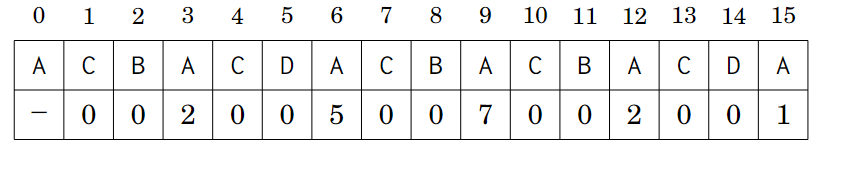
\includegraphics[width=\linewidth]{string_z_algorithm_01.png}
\end{figure}

Es este caso, para el ejemplo, $z[6]\:=\:5$, porque el substring $ACBAC$ de longitud $5$ es un prefijo de $s$, pero para el substring $ACBACB$ de longitud $6$ no es un prefijo de $s$.

\begin{lstlisting}
// z_array=length of the longest substring starting from s[i] which is also a prefix of s
vector<int> z_algorithm(const string &s) {
    int n = (int) s.size();
    vector<int> z_array(n);
    int left=0, right=0;
    z_array[0] = 0;
    for(int idx = 1; idx < n; ++idx) {
        z_array[idx] = max(0, min(z_array[idx-left], right-idx+1));
        while (idx+z_array[idx] < n && s[z_array[idx]] == s[idx+z_array[idx]]) {
            left = idx;
            right = idx + z_array[idx];
            z_array[idx]++;
        }
    }
    return z_array;
}
\end{lstlisting}

\subsection{Aho Corasick}
\begin{lstlisting}
// El trie (o prefix tree) guarda un diccionario de strings como un arbol enraizado.
// Aho corasick permite encontrar las ocurrencias de todos los strings del trie en un string s.

const int alpha = 26; // cantidad de letras del lenguaje
const char L = 'a'; // primera letra del lenguaje

struct node {
    int next[alpha], end;
    int link, exit, cnt;
    int& operator[](int i) { return next[i]; }
};

vector<node> trie = {node()};

void add_str(string &s, int id = 1) {
    int u = 0;
    for (auto ch : s) {
        int c = ch-L;
        if (!trie[u][c]) {
            trie[u][c] = trie.size();
            trie.push_back(node());
        }
        u = trie[u][c];
    }
    trie[u].end = id; //con id > 0
    trie[u].cnt++;
}

// aho corasick
void build_ac() {
    queue<int> q; q.push(0);
    while (q.size()) {
        int u = q.front(); q.pop();
        for (int c = 0; c < alpha; ++c) {
            int v = trie[u][c];
            if (!v) trie[u][c] = trie[trie[u].link][c];
            else q.push(v);
            if (!u || !v) continue;
            trie[v].link = trie[trie[u].link][c];
			trie[v].exit = trie[trie[v].link].end ? trie[v].link : trie[trie[v].link].exit;
            trie[v].cnt += trie[trie[v].link].cnt;
        }
    }
}

vector<int> cnt; //cantidad de ocurrencias en s para cada patron

void run_ac(string &s) {
    int u = 0, sz = s.size();
    for (int i = 0; i < sz; ++i) {
        int c = s[i]-L;
        while (u && !trie[u][c]) u = trie[u].link;
        u = trie[u][c];
        int x = u;
        while (x) {
            int id = trie[x].end;
            if (id) cnt[id-1]++;
            x = trie[x].exit;
        }
    }
}
\end{lstlisting}


% MATH
\section{Math}

\subsection{Diophantine}
\begin{lstlisting}
// Use extgcd
template<typename T>
bool diophantine(T a, T b, T c, T & x, T & y, T & g) {
    if (a == 0 && b == 0) {
        if (c == 0) {
            x = y = g = 0;
            return true;
        }
        return false;
    }
    auto [g1, x1, y1] = extgcd(a, b);
    if (c % g1 != 0)
        return false;
    g = g1;
    x = x1 * (c / g);
    y = y1 * (c / g);
    return true;
}
// Usage
// int x, y, g;
// bool can = diophantine(a, b, c, x, y, g);

// a*x + b*y = c -> If and only if gcd(a, b) is a divisor of c
\end{lstlisting}

\subsection{Divisors}
\begin{lstlisting}
template<typename T>
vector<T> divisors(T number) {
    vector<T> ans;
    for (T i = 1; i*i <= number; ++i) {
        if (number % i == 0) {
            if (number/i == i) {
                // if i*i == number
                ans.push_back(i);
            } else {
                // x=i, y=number/i, if x*y==number
                ans.push_back(i);
                ans.push_back(number/i);
            }
        }
    }
    return ans;
}
\end{lstlisting}

\subsection{Ext GCD}
\begin{lstlisting}
template<typename T>
tuple<T, T, T> extgcd(T a, T b) {
    if (a == 0)
        return {b, 0, 1};
    T p = b / a;
    auto [g, y, x] = extgcd(b - p * a, a);
    x -= p * y;
    return {g, x, y};
}
// Usage:
//   auto [g, x, y] = extgcd(a, b);

// a*x ≡ 1 (mod m) -> If and only if gcd(a, m) == 1
// a*x + m*y = 1

// auto [g, x, y] = extgcd(a, m);

// a*x + b*y = gcd(a, b) 
\end{lstlisting}

\subsection{GCD}
\begin{lstlisting}
template<class T>
T gcd(T a, T b) {
    return (b == 0)?a:gcd(b, a % b);
}
\end{lstlisting}

\subsection{LCM}
\begin{lstlisting}
template<class T>
T lcm(T a, T b) {  
    return (a*b)/gcd<T>(a, b);  
}
\end{lstlisting}

\subsection{Matrix}
\begin{lstlisting}
// Estructura para realizar operaciones de multiplicacion y exponenciacion modular sobre matrices.

const int mod = 1e9+7;

struct matrix {
    vector<vector<int>> v;
    int n, m;
    
    matrix(int n, int m, bool o = false) : n(n), m(m), v(n, vector<int>(m)) {
        if (o) while (n--) v[n][n] = 1;
    }

    matrix operator * (const matrix &o) {
        matrix ans(n, o.m);
        for (int i = 0; i < n; i++)
            for (int k = 0; k < m; k++) if (v[i][k])
                for (int j = 0; j < o.m; j++)
                    ans[i][j] = (1LL * v[i][k] * o.v[k][j] + ans[i][j]) % mod;
        return ans;
    }
    
    vector<int>& operator[] (int i) { return v[i]; }
};

matrix pow(matrix b, ll e) {
    matrix ans(b.n, b.m, true);
    while (e) {
        if (e&1) ans = ans*b;
        b = b*b;
        e /= 2;
    }
    return ans;
}
\end{lstlisting}

\subsection{Lineal Recurrences}
\begin{lstlisting}
// Calcula el n-esimo termino de una recurrencia lineal (que depende de los k terminos anteriores).
// * Llamar init(k) en el main una unica vez si no es necesario inicializar las matrices multiples veces.
// Este ejemplo calcula el fibonacci de n como la suma de los k terminos anteriores de la secuencia (En la secuencia comun k es 2).
// Agregar Matrix Multiplication con un construcctor vacio.

matrix F, T;

void init(int k) {
    F = {k, 1}; // primeros k terminos
    F[k-1][0] = 1;
    T = {k, k}; // fila k-1 = coeficientes: [c_k, c_k-1, ..., c_1]
    for (int i = 0; i < k-1; i++) T[i][i+1] = 1;
    for (int i = 0; i < k; i++) T[k-1][i] = 1;
}

/// O(k^3 log(n))
int fib(ll n, int k = 2) {
    init(k);
    matrix ans = pow(T, n+k-1) * F;
    return ans[0][0];
}
\end{lstlisting}

\subsection{Phi Euler}
\begin{lstlisting}
template<typename T>
T phi_euler(T number) {
    T result = number;
    for(T i = static_cast<T>(2); i*i <= number; ++i) {
        if(number % i != 0)
            continue;
        while(number % i == 0) {
            number /= i;
        }
        result -= result / i;
    }
    if(number > 1)
        result -= result / number;
    return result;
}
\end{lstlisting}

\subsection{Primality Test}
\begin{lstlisting}
template<typename T>
bool is_prime(T number) {
    if(number <= 1)
        return false;
    else if(number <= 3)
        return true;
    if(number%2==0 || number%3==0)
        return false;
    for(T i = 5; i*i <= number; i += 6) {
        if(number%i==0 || number%(i+2)==0)
            return false;
    }
    return true;
    // Time Complexity: O(sqrt(N)), Space Complexity:  O(1)
}
\end{lstlisting}

\subsection{Primality Test Miller Rabin}
\begin{lstlisting}
// Reference: notebook_descomUNAL
ll mul (ll a, ll b, ll mod) {
    ll ret = 0;
    for(a %= mod, b %= mod; b != 0;
      b >>= 1, a <<= 1, a = a >= mod ? a - mod : a) {
        if (b & 1) {
            ret += a;
            if (ret >= mod) ret -= mod;
        }
    }
    return ret;
}
ll fpow (ll a, ll b, ll mod) {
    ll ans = 1;
    for (; b; b >>= 1, a = mul(a, a, mod))
        if (b & 1)
            ans = mul(ans, a, mod);
    return ans;
}
bool witness (ll a, ll s, ll d, ll n) {
    ll x = fpow(a, d, n);
    if (x == 1 || x == n - 1) return false;
    for (int i = 0; i < s - 1; i++) {
        x = mul(x, x, n);
        if (x == 1) return true;
        if (x == n - 1) return false;
    }
    return true;
}
ll test[] = {2, 3, 5, 7, 11, 13, 17, 19, 23, 0};
bool is_prime (ll n) {
    if (n < 2) return false;
    if (n == 2) return true;
    if (n % 2 == 0) return false;
    ll d = n - 1, s = 0;
    while (d % 2 == 0) ++s, d /= 2;
    for (int i = 0; test[i] && test[i] < n; ++i)
        if (witness(test[i], s, d, n))
            return false;
    return true;
}
\end{lstlisting}

\subsection{Prime Factos}
\begin{lstlisting}
template<class T>
map<T, int> prime_factors(T number)  {
    map<T, int> factors;
    while (number % 2 == 0) {
        factors[2]++;
        number = number / 2;
    }
    for (T i = 3; i*i <= number; i += 2) {
        while (number % i == 0) {
            factors[i]++;
            number = number / i; 
        }
    }
    if (number > 2)
        factors[number]++;
    return factors;
}
//   for n=100, { 2: 2, 5: 2}
//   2*2*5*5 = 2^2 * 5^2 = 100
\end{lstlisting}

\subsection{Sieve}
\begin{lstlisting}
using int64 = long long;

const int mxN = 1e6;
bool marked[mxN+1];
vector<int> primes;
/// O(mxN log(log(mxN)))
void sieve() {
    marked[0] = marked[1] = true;
    for (int i = 2; i <= mxN; i++) {
        if (marked[i]) continue;
        primes.push_back(i);
        for (int64 j = 1LL * i*i; j <= mxN; j += i)
            marked[j] = true;
    }
}
\end{lstlisting}

\subsection{Math Utils}
\begin{lstlisting}
#define PI   3.141592653589793238462643383279502884L // acos(-1);
#define E    2.718281828459045235360287471352662497L
#define eps  1e-9

template<typename T>
int cmp(const T &a, const T &b) {
    return ( (a + eps < b)? -1 :( (b + eps < a )? 1 : 0) );
}

template<typename T>
T ceiling_division(T numerator, T denominator) {
    assert(denominator != static_cast<T>(0));
    return (numerator+denominator-1)/denominator;
}

// How much does it need to add to n so that it is divisible by k
template<typename T>
T distance_divisible(T n, T k) {
    assert(0 < k); if(n < k) return k - n % k;
    return n % k;
}
\end{lstlisting}

% DYNAMIC PROGRAMMING

\section{Dynamic Programming}

\subsection{Diameter dp on tree}
\begin{lstlisting}
const int mxN = 2e5 + 10;
vector<int> adj[mxN];
int n;
 
int dist[mxN];
int dp[mxN];
 
int dfs(int node, int parent) {
    dist[node] = 0;
    int mx_dist = 0;
    int first = -1, second = -1;
    for(auto &child: adj[node]) {
        if(child == parent)
            continue;
        mx_dist = max(mx_dist, dfs(child, node) + 1);
        if(dist[child] >= first) {
            if(first != -1) second = first;
            first = dist[child];
        } else if(dist[child] >= second) {
            second = dist[child];
        }
    }
    dist[node] = mx_dist;
    dp[node] = first + second + 2;
    return mx_dist;
}
// undigraph
// dfs(0, -1);
// int diameter = *max_element(dp, dp + n);
\end{lstlisting}

\subsection{DP on Directed Acyclic Graph}
\begin{lstlisting}
// Problemas clasicos con DAG
const int INF = 1e9;
const int MAX = 1000;
int init, fin;
int dp[MAX];
vector<int> g[MAX]; // USADO PARA ARISTAS NO PONDERADAS
vector<pair<int, int>> gw[MAX]; // PARA ARISTAS PONDERADAS First: Nodo vecino. Second = Peso de la arista
// Funcion para calcular el numero de formas de ir del nodo u al nodo end
// LLamar para nodo inicial (init)
int ways(int u){
    if(u == fin) return 1;
    int &ans = dp[u];
    if(ans != -1) return ans;
    ans = 0;
    for(auto v: g[u]){
        ans += ways(v);
    }
    return ans;
}
// MINIMO CAMINO DESDE U HASTA END. LLAMAR PARA INIT
int min_way(int u){
    if(u == fin) return 0;
    int &ans = dp[u];
    if(ans != -1) return ans;
    ans = INF;
    for(auto v: gw[u]){
        ans = min(ans, min_way(v.first) + v.second);
    }
    return ans;
}
\end{lstlisting}

\subsection{Edit Distance}
\begin{lstlisting}
int edit_dist(string &s1, string &s2, int m, int n) {
    // If first string is empty, the only option is to
    // insert all characters of second string into first
    if (m == 0) return n;

    // If second string is empty, the only option is to
    // remove all characters of first string
    if (n == 0)
        return m;
 
    // If last characters of two strings are same, nothing
    // much to do. Ignore last characters and get count for
    // remaining strings.
    if (s1[m - 1] == s2[n - 1])
        return edit_dist(s1, s2, m - 1, n - 1);
 
    // If last characters are not same, consider all three
    // operations on last character of first string,
    // recursively compute minimum cost for all three
    // operations and take minimum of three values.
    return 1 + min({
        edit_dist(s1, s2, m, n - 1),    // Insert
        edit_dist(s1, s2, m - 1, n),    // Remove
        edit_dist(s1, s2, m - 1, n - 1) // Replace
    });
}
\end{lstlisting}

\subsection{Snapsack}
\begin{lstlisting}
vector<vector<int64>> dp;

int64 knapsack(vector<int64> &val, vector<int64> &wt, int item, int capacity) {
    // Casos base
    if(item <= 0 || capacity <= 0) return 0;

    if(dp[item][capacity] != -1) return dp[item][capacity];
    
    int itemCurr = item - 1;
    // Maximos items acumulado
    int64 lastMax = knapsack(val, wt, item-1, capacity);
    int64 currMax = 0;

    if(wt[itemCurr] <= capacity) {
        // Valor del item actual + el mejor item que cabe en la mochila
        currMax = val[itemCurr] + knapsack(val, wt, item - 1, capacity-wt[itemCurr]);
    }

    dp[item][capacity] = max(lastMax, currMax);
    return dp[item][capacity];
}
// vector<int> val{10, 40, 30, 50};
// vector<int> wt{5, 4, 6, 3};
// int n = val.size();
// int w = 10;
// knapsack(val, wt, n, w)
\end{lstlisting}

\subsection{Longest Common Subsecuence}
\begin{lstlisting}
// Longest Common Subsecuence
int lcs(string X, string Y, int m, int n) {
    if (m == 0 || n == 0) {
        return 0;
    }
    if (X[m - 1] == Y[n - 1]) {
        return 1 + lcs(X, Y, m - 1, n - 1);
    }
    return max(lcs(X, Y, m, n - 1), lcs(X, Y, m - 1, n));
}
\end{lstlisting}

\subsection{Longest Increasing Subsecuence - DP}
\begin{lstlisting}
int lis(int arr[], int i, int n, int prev) {
    // Base case: nothing is remaining
    if (i == n) {
        return 0;
    }
    int excl = lis(arr, i + 1, n, prev); 
    int incl = 0;
    if (arr[i] > prev) {
        incl = 1 + lis(arr, i + 1, n, arr[i]);
    }
    return max(incl, excl);
}
\end{lstlisting}

\subsection{Longest Increasing Subsecuence - Optimization}
\begin{lstlisting}
// Longest Increasing Subsequence O(n*lg(n))
template <typename T>
int lis(const vector<T> &a) {
    vector<T> u;
    for (const T &x : a) {
        auto it = lower_bound(u.begin(), u.end(), x);
        if (it == u.end()) {
            u.push_back(x);
        } else {
            *it = x;
        }
    }
    return (int) u.size();
}
// LIS O(nlog(n)) Para longest non-decreasing cambiar lower_bound por upper_bound
int lis(){
    LIS.clear();
    for(int i = 0; i < N; i++){
        auto id = lower_bound(LIS.begin(), LIS.end(), A[i]);
        if(id == LIS.end()){
            LIS.push_back(A[i]);
            dp[i] = LIS.size();
        } 
        else{
            int idx = id - LIS.begin();
            LIS[idx] = A[i];
            dp[i] = idx + 1;
        }
    }
    return LIS.size();
}
// METODO PARA RECONSTRUIR LIS. Para non-decreasing cambiar < por <=
stack<int> rb;
void build(){
    int k = LIS.size();
    int cur = oo;
    for(int i = N - 1; i >= 0, k; i--){
        if(A[i] < cur && k == dp[i]){
            cur = A[i];
            rb.push(A[i]);
            k--;
        }
    }
}
\end{lstlisting}

% Search
\section{Search}

\subsection{Binary Search - I}
\begin{lstlisting}
int n = oo;
int low = 0, high = n, mid;
while (high - low > 1) {
    mid = low + (high - low) / 2;
    if(!ok(mid)) {
        low = mid;
    } else {
        high = mid;
    }
}
// low or high
\end{lstlisting}

\subsection{Binary Search - II}
\begin{lstlisting}
int n = oo;
int index = -1;
for(int jump = n+1; jump >= 1; jump /= 2) {
    while(jump+index<n && !ok(jump+index)) {
        index += jump;
    }
}
// index + 1
\end{lstlisting}

\subsection{Binary Search on Real Values - I}
\begin{lstlisting}
double eps = 1e-9;
double n = inf;
double low = 0.0, high = n, mid;
while ((high - low) > eps) {
    mid = double(high + low) / 2.0;
    if(!ok(mid)) {
        low = mid;
    } else {
        high = mid;
    }
}
// low or high
\end{lstlisting}

\subsection{Binary Search on Real Values - II}
\begin{lstlisting}
double n = inf;
double low = 0.0, high = n, mid;
int iter = 0;
while(iter < 300) {
    mid = double(high + low) / 2.0;
    if(!ok(mid)) {
        low = mid;
    } else {
        high = mid;
    }
    iter++;
}
// low or high
\end{lstlisting}

\subsection{Merge Sort}
\begin{lstlisting}
void merge(vector<int> &v, int left, int mid, int right) {
    vector<int> ordered(right-left+1);
    int i = left, j = mid + 1, idx = 0;
    while(i <= mid ||  j <= right) {
        if(i <= mid && j <= right) {
            if(v[i] < v[j]) {
                ordered[idx++] = v[i++];    
            } else if(v[i] > v[j]) {
                ordered[idx++] = v[j++];
            } else {
                ordered[idx++] = v[i++];
                ordered[idx++] = v[j++];
            }
        } else if(i <= mid) {
            ordered[idx++] = v[i++];
        } else if(j <= right) {
            ordered[idx++] = v[j++];
        }
    }
    for(idx=0, i = left; i <= right; i++)
        v[i] = ordered[idx++];
}
void merge_sort(vector<int> &v, int left, int right) {
    if(left == right) {
        return;
    } else if(left < right) {
        int mid = (left+right)/2;
        merge_sort(v, left, mid);
        merge_sort(v, mid+1, right);
        merge(v, left, mid, right);    
    }
}
void merge_sort(vector<int> &v) {
    merge_sort(v, 0, (int) v.size() - 1);
}
// Usage:
// Vector<int> A { ... };
// merge_sort(A);
\end{lstlisting}

% TECHNIQUES
\section{Techniques}

\subsection{Divide and Conquer}
\begin{lstlisting}
void divide(int left, int right) {
    if(left == right) {
        return;
    } else if(left < right) {
        int mid = (left + right) / 2;
        divide(left, mid);
        divide(mid+1, right);
    }
}
\end{lstlisting}

\subsection{Mo's Algorithm}
\begin{lstlisting}
// Complexity: O(|N+Q|*sqrt(|N|)*|add+del|)

struct Query {
    int left, right, index;
    Query (int l, int r, int idx)
        : left(l), right(r), index(idx) {}
};

int S; // S = sqrt(n);

bool cmp (const Query &a, const Query &b) {
    if (a.left/S != b.left/S)
        return a.left/S < b.left/S;
    return a.right > b.right;
}

// global functions
void add(int idx) {

}
void del(int idx) {

}
auto get_answer() {

}

// at main()
vector<Query> Q;
Q.reserve(q+1);
int from, to;
for(int i = 0; i < q; ++i){
    cin >> from >> to; // don't forget (from--, to--) if it's 1-indexed
    Q.push_back(Query(from, to, i));
}

S = sqrt(n); // n = size of array
sort(Q.begin(), Q.end(), cmp);

vector<int> ans(q);
int left = 0, right = -1;

for (int i = 0; i < (int) Q.size(); ++i) {
    while (right < Q[i].right)
        add(++right);
    while (left > Q[i].left)
        add(--left);
    while (right > Q[i].right)
        del(right--);
    while (left < Q[i].left)
        del(left++);
    
    ans[Q[i].index] = get_answer();
}
\end{lstlisting}

\subsection{Sliding Windows}
\begin{lstlisting}
// sequence: [a1, a2, a3, a4, a5, a6, a7,  ..., an]
//                |<- sliding window ->|
//                v                    v 
//             [start]-->            [end]-->

// int n = (int) any.size();
// int start=0, end=0;
// map<int, int> counter;
// int ans = 0;
// while(end < n) {
//     counter[any[end]]++;
//     while(condition(start, end) && start <= end) {
//         counter[any[start]]--;
//         process_logic1(start,end);
//         start++;
//     }
//     process_logic2(start,end);
//     ans = max(ans, end - start + 1);
//     end++;
// }
// print(ans);
\end{lstlisting}

\subsection{Sweep Line}
\begin{lstlisting}
struct Event {
    int time, delta, idx;
    bool operator<(const Event &other) const { return time < other.time; }
};

// Usage:
// vector<Event> events;
// events.reserve(2*n);
// int from, to;
// for(int i = 0; i < n; ++i) {
//     read from and to values
//     events.push_back(Event{from, 1, i});
//     events.push_back(Event{to, -1, i});
// }
// sort(events.begin(), events.end());
// for(const auto &event: events) {
//     process_logic(event.delta); for example
//     total += event.delta;
//     best = max(best, total);
// }
\end{lstlisting}

\subsection{Two Pointer Left Right Boundary}
\begin{lstlisting}
// sequence:  [a1, a2, a3, a4, ..., an]
//     [left] ->->              <-<-<- [right]

// int left=0, right=n-1;
// while(left < right) {
//     if(left_condition(left)) {
//         left++;
//     }
//     if(right_condition(right)) {
//         right--;
//     }
//     process_logic(left, right);
// }
\end{lstlisting}

\subsection{Two Pointer1 Pointer2}
\begin{lstlisting}
// seq1: [a1, a2, a3, ..., an]
// [p1] ->->->->->

// seq2: [b1, b2, b3, ..., bn]
// [p2] ->->

// int n = (int) seq1.size();
// int m = (int) seq2.size();
// int p1=0, p2=0; // or seq1[0], seq2[0]
// while(p1 < n && p2 < m) {
//     if(p1_condition(p1)) {
//         p1++;
//     }
//     if(p2_condition(p2)) {
//         p2++;
//     }
//     process_logic(p1, p2);
// }
\end{lstlisting}

\subsection{Two Pointers Old And New State}
\begin{lstlisting}
// sequence:             [ a1,   a2,   a3, ...]
//                         |      |    |
//                         v      v    v
// new state:      [new0,  new1, new2, new3, ...]
//                    |     |      |
//                    v     v      v
// new state: [old0, old1, old2,  old3, ...]

// new state:       [old0,  old1,  old2, old3, ...]
//                    |      |      |
//                    v      v      v
// new state: [new0, new1, new2,  new3, ...]

// int last = default_val1;
// int now = default_val2;
// for(int i = 0; i < n; ++i){
//     last =  now;
//     now = process_logic(element, old)
// }
\end{lstlisting}

\subsection{Two Pointers Slow Fast}
\begin{lstlisting}
// sequence: [a1, a2, a3, ..., an]
// slow runner: [slow] ->->
// fast runner: [fast] ->->->->

// int slow = 0;
// for(int fast = 0; fast < n; ++fast){
//     if(slow_condition(slow)) {
//         slow = slow.next;
//         slow += 1;
//     }
//     process_logic(slow, fast);
// }
\end{lstlisting}


% COMBINATORICS
\section{Combinatorics}

\subsection{All Combinations Backtracking}
\begin{lstlisting}
vector<vector<int>> answer;
vector<int> combination;
void combinations_backtraking(const int &n, const int &k,  int idx) {
    if(idx == k) {
        answer.push_back(combination);
        return;
    }
    int start = (combination.size()==0)?1:combination.back()+1;
    for(int i = start; i <= n; ++i) {
        combination.push_back(i);
        combinations_backtraking(n, k, idx+1);    
        combination.pop_back();
    }
}
\end{lstlisting}

\subsection{Binomial Coefficient}
Calcula el coeficiente binomial nCr, entendido como el numero de subconjuntos de r elementos escogidos de un conjunto con n elementos.

\begin{lstlisting}
// O(min(r, n-r))
int64 nCr(int64 n, int64 r) {
    if (r < 0 || n < r) return 0;
    r = min(r, n-r);
    int64 ans = 1;
    for (int i = 1; i <= r; i++) {
        ans = ans * (n-i+1) / i;
    }
    return ans;
}
\end{lstlisting}

\subsection{Kth Permutation}
\begin{lstlisting}
vector<int> kth_permutation(vector<int> perm, int  k) {
    int64_t factorial = 1LL;
    int n = (int) perm.size();
    for(int64_t num = 2; num < n; ++num)
        factorial *= num; // (n-1)!
    k--; // k-th to 0-indexed
    vector<int> answer; answer.reserve(n);
    while(true) {
        answer.push_back(perm[k / factorial]);
        perm.erase(perm.begin()+(k/factorial));
        if((int) perm.size() == 0)
            break;
        k %= factorial;
        factorial /= (int) perm.size();
    }
    return answer;
}

vector<int> kth_permutation(int n, int k, int start=0) {
    vector<int> perm(n);
    iota(perm.begin(), perm.end(), start);
    return kth_permutation(perm, k);
}

string kth_perm_string(int n, int k) {
    assert(1 <= n && n <= 26);
    vector<int> perm = kth_permutation(n, k);
    string alpha = "";
    for(char i='a'; i <= ('a'+n); ++i)
        alpha.push_back(i);
    string answer="";
    for(int &idx: perm)
        answer.push_back(alpha[idx]);
    return answer;
}
\end{lstlisting}

\subsection{Next Combination}
this works for 1 <= k <= n <= 20 approximately
Complexity: worst case $O(2^n)$ approximately
\begin{lstlisting}
bool next_combination(vector<int> &comb, int n) {
    int k = (int) comb.size();
    for (int i = k - 1; i >= 0; i--) {
        if (comb[i] <= n - k + i) {
            ++comb[i];
            while (++i < k) {
                comb[i] = comb[i - 1] + 1;
            }
            return true;
        }
    }
    return false;
}

void all_combinations(int n, int k) {
    vector<int> comb(k);
    iota(comb.begin(), comb.end(), 1);
    do {
        for (const int &v : comb) {
            cout << v << " ";
        }
        cout << endl;
    } while (next_combination(comb, n));
}
\end{lstlisting}

% NUMERICS
\section{Numerics}

\subsection{Fastpow}
\begin{lstlisting}
template<typename T, typename U>
T fastpow(T a, U b) {
    assert(0 <= b);
    T ans = static_cast<T>(1);
    while (b > 0) {
        if (b & 1) ans = ans*a;
        a *= a;
        b >>= 1;
    }
    return ans;
}
\end{lstlisting}

\subsection{Numeric Mod}
\begin{lstlisting}
const int MOD = int(1e9+7);

template<typename T>
T sub(T a, T b) {
    return (1LL*(a-b)%MOD + MOD) % MOD;
}
template<typename T>
T add(T a, T b) {
    return (1LL*(a%MOD) + 1LL*(b%MOD)) % MOD;
}
template<typename T>
T mul(T a, T b) {
    return (1LL*(a%MOD) * (b%MOD)) % MOD;
}
template<typename T, typename U>
T fastpow(T a, U b) {
    assert(0 <= b);
    T answer = static_cast<T>(1);
    while (b > 0) {
        if (b & 1) {
            answer = mul(answer, a);
        }
        a = mul(a, a);
        b >>= 1;
    }
    return answer;
}
template<typename T>
T inverse(T a) {
    a %= MOD;
    if (a < 0) a += MOD;
    T b = MOD, u = 0, v = 1;
    while (a) {
        T t = b / a;
        b -= t * a; swap(a, b);
        u -= t * v; swap(u, v);
    }
    assert(b == 1);
    if (u < 0) u += MOD;
    return u;
}
template<typename T>
T division(T a, T b) {
    return mul(a, inverse(b));
}
\end{lstlisting}


% BIT MASK
\section{Bit Mask}

\subsection{Tricks}
\begin{lstlisting}
int zeros_left(int num) {return (num==0)?32:__builtin_clz(num);}
int zeros_right(int num) {return (num==0)?0:__builtin_ctz(num);}
int count_ones(int num) {return __builtin_popcount(num);}
int parity(int num) {return __builtin_parity(num);}
int LSB(int num) {return __builtin_ffs(num);} //  Least Significant Bit [0 if num == 0]
 
int64_t zeros_left(int64_t num) {return (num==0LL)?64LL:__builtin_clzll(num);}
int64_t zeros_right(int64_t num) {return (num==0LL)?0LL:__builtin_ctzll(num);}
int64_t count_ones(int64_t num) {return __builtin_popcountll(num);}
int64_t parity(int64_t num) {return __builtin_parityll(num);}
int64_t LSB(int64_t num) {return __builtin_ffsll(num);} //  Least Significant Bit [0 if number == 0]
 
template<typename T>
int hamming(const T &lhs, const T &rhs) {
    if(is_same<T, int64_t>::value) return __builtin_popcountll(lhs ^ rhs);
    return __builtin_popcount(lhs ^ rhs);
}

// 1LL for 64-bits

// x & 1            : Check if x is odd
// x & (1 << i)     : Check if the i-th bit is HIGH
// x = x | (1<<i)   : Set HIGH i-th bit
// x = x & ~(1<<i)  : Set LOW i-th bit
// x = x ^ (1<<i)   : Flip i-th bit
// x = ~x           : Flip all the bits
// x & -x           : returns the number of the first HIGH bit from right to left (power of 2, not the index)
// log2(x & -x)     : Return position of first bit HIGH from right to left (0-index [..., 3, 2, 1, 0])
// ~x & (x+1)       : Returns the number of the first LOW bit from right to left (power of 2, not the index)
// log2(~x & (x+1)) : Returns position of the first LOW bit from right to left (0-index [..., 3, 2, 1, 0])
// x = x | (x+1)    : Set HIGH of first bit from right to left
// x = x & (x-1)    : Set LOW of first bit from right to left
// x = x & ~y       : Set LOW in x the HIGH bits in y

// Iterates over the indices of the high bits in a mask
/// O(#bits_encendidos)
// for (int x = mask; x; x &= x-1) {
//     int i = __builtin_ctz(x);
// }

// Iterate all the submasks of a mask. (Iterate all submasks of all masks is O(3^n)).
/// O(2^(#bits_encendidos))
// for (int sub = mask; sub; sub = (sub-1)&mask) {
// }
\end{lstlisting}

% GEOMETRY

\section{Geometry}

\subsection{Geometry Template}
\begin{lstlisting}
const lf eps = 1e-9;
typedef double T;
struct pt {
  T x, y;
  pt operator + (pt p) { return {x+p.x, y+p.y}; }
  pt operator - (pt p) { return {x-p.x, y-p.y}; }
  pt operator * (pt p) { return {x*p.x-y*p.y, x*p.y+y*p.x}; }
  pt operator * (T d) { return {x*d, y*d}; }
  pt operator / (lf d) { return {x/d, y/d}; } /// only for floating point
  bool operator == (pt b) { return x == b.x && y == b.y; }
  bool operator != (pt b) { return !(*this == b); }
  bool operator < (const pt &o) const { return y < o.y || (y == o.y && x < o.x); }
  bool operator > (const pt &o) const { return y > o.y || (y == o.y && x > o.x); }
};
int cmp (lf a, lf b) { return (a + eps < b ? -1 :(b + eps < a ? 1 : 0)); }
/** Already in complex **/
T norm(pt a) { return a.x*a.x + a.y*a.y; }
lf abs(pt a) { return sqrt(norm(a)); }
lf arg(pt a) { return atan2(a.y, a.x); }
ostream& operator << (ostream& os, pt &p) {
  return os << "("<< p.x << "," << p.y << ")";
}
/***/
istream &operator >> (istream &in, pt &p) {
    T x, y; in >> x >> y;
    p = {x, y};
    return in;
}
T dot(pt a, pt b) { return a.x*b.x + a.y*b.y; }
T cross(pt a, pt b) { return a.x*b.y - a.y*b.x; }
T orient(pt a, pt b, pt c) { return cross(b-a,c-a); }
//pt rot(pt p, lf a) { return {p.x*cos(a) - p.y*sin(a), p.x*sin(a) + p.y*cos(a)}; }
//pt rot(pt p, double a) { return p * polar(1.0, a); } /// for complex
//pt rotate_to_b(pt a, pt b, lf ang) { return rot(a-b, ang)+b; }
pt rot90ccw(pt p) { return {-p.y, p.x}; }
pt rot90cw(pt p) { return {p.y, -p.x}; }
pt translate(pt p, pt v) { return p+v; }
pt scale(pt p, double f, pt c) { return c + (p-c)*f; }
bool are_perp(pt v, pt w) { return dot(v,w) == 0; }
int sign(T x) { return (T(0) < x) - (x < T(0)); }
pt unit(pt a) { return a/abs(a); }

bool in_angle(pt a, pt b, pt c, pt x) {
  assert(orient(a,b,c) != 0);
  if (orient(a,b,c) < 0) swap(b,c);
  return orient(a,b,x) >= 0 && orient(a,c,x) <= 0;
}

//lf angle(pt a, pt b) { return acos(max(-1.0, min(1.0, dot(a,b)/abs(a)/abs(b)))); }
//lf angle(pt a, pt b) { return atan2(cross(a, b), dot(a, b)); }
/// returns vector to transform points
pt get_linear_transformation(pt p, pt q, pt r, pt fp, pt fq) {
  pt pq = q-p, num{cross(pq, fq-fp), dot(pq, fq-fp)};
  return fp + pt{cross(r-p, num), dot(r-p, num)} / norm(pq);
}

bool half(pt p) { /// true if is in (0, 180]
  assert(p.x != 0 || p.y != 0); /// the argument of (0,0) is undefined
  return p.y > 0 || (p.y == 0 && p.x < 0);
}
bool half_from(pt p, pt v = {1, 0}) {
  return cross(v,p) < 0 || (cross(v,p) == 0 && dot(v,p) < 0);
}
bool polar_cmp(const pt &a, const pt &b) {
  return make_tuple(half(a), 0) < make_tuple(half(b), cross(a,b));
}

struct line {
  pt v; T c;
  line(pt v, T c) : v(v), c(c) {}
  line(T a, T b, T c) : v({b,-a}), c(c) {}
  line(pt p, pt q) : v(q-p), c(cross(v,p)) {}
  T side(pt p) { return cross(v,p)-c; }
  lf dist(pt p) { return abs(side(p)) / abs(v); }
  lf sq_dist(pt p) { return side(p)*side(p) / (lf)norm(v); }
  line perp_through(pt p) { return {p, p + rot90ccw(v)}; }
  bool cmp_proj(pt p, pt q) { return dot(v,p) < dot(v,q); }
  line translate(pt t) { return {v, c + cross(v,t)}; }
  line shift_left(double d) { return {v, c + d*abs(v)}; }
  pt proj(pt p) { return p - rot90ccw(v)*side(p)/norm(v); }
  pt refl(pt p) { return p - rot90ccw(v)*2*side(p)/norm(v); }
};

bool inter_ll(line l1, line l2, pt &out) {
  T d = cross(l1.v, l2.v);
  if (d == 0) return false;
  out = (l2.v*l1.c - l1.v*l2.c) / d;
  return true;
}
line bisector(line l1, line l2, bool interior) {
  assert(cross(l1.v, l2.v) != 0); /// l1 and l2 cannot be parallel!
  lf sign = interior ? 1 : -1;
  return {l2.v/abs(l2.v) + l1.v/abs(l1.v) * sign,
          l2.c/abs(l2.v) + l1.c/abs(l1.v) * sign};
}

bool in_disk(pt a, pt b, pt p) {
  return dot(a-p, b-p) <= 0;
}
bool on_segment(pt a, pt b, pt p) {
  return orient(a,b,p) == 0 && in_disk(a,b,p);
}
bool proper_inter(pt a, pt b, pt c, pt d, pt &out) {
  T oa = orient(c,d,a),
  ob = orient(c,d,b),
  oc = orient(a,b,c),
  od = orient(a,b,d);
  /// Proper intersection exists iff opposite signs
  if (oa*ob < 0 && oc*od < 0) {
    out = (a*ob - b*oa) / (ob-oa);
    return true;
  }
  return false;
}
set<pt> inter_ss(pt a, pt b, pt c, pt d) {
  pt out;
  if (proper_inter(a,b,c,d,out)) return {out};
  set<pt> s;
  if (on_segment(c,d,a)) s.insert(a);
  if (on_segment(c,d,b)) s.insert(b);
  if (on_segment(a,b,c)) s.insert(c);
  if (on_segment(a,b,d)) s.insert(d);
  return s;
}
lf pt_to_seg(pt a, pt b, pt p) {
  if(a != b) {
    line l(a,b);
    if (l.cmp_proj(a,p) && l.cmp_proj(p,b)) /// if closest to  projection
      return l.dist(p); /// output distance to line
  }
  return min(abs(p-a), abs(p-b)); /// otherwise distance to A or B
}
lf seg_to_seg(pt a, pt b, pt c, pt d) {
  pt dummy;
  if (proper_inter(a,b,c,d,dummy)) return 0;
  return min({pt_to_seg(a,b,c), pt_to_seg(a,b,d),
              pt_to_seg(c,d,a), pt_to_seg(c,d,b)});
}

enum {IN, OUT, ON};
struct polygon {
  vector<pt> p;
  polygon(int n) : p(n) {}
  int top = -1, bottom = -1;
  void delete_repetead() {
    vector<pt> aux;
    sort(p.begin(), p.end());
    for(pt &i : p)
      if(aux.empty() || aux.back() != i)
        aux.push_back(i);
    p.swap(aux);
  }
  bool is_convex() {
    bool pos = 0, neg = 0;
    for (int i = 0, n = p.size(); i < n; i++) {
      int o = orient(p[i], p[(i+1)%n], p[(i+2)%n]);
      if (o > 0) pos = 1;
      if (o < 0) neg = 1;
    }
    return !(pos && neg);
  }
  lf area(bool s = false) {
    lf ans = 0;
    for (int i = 0, n = p.size(); i < n; i++)
      ans += cross(p[i], p[(i+1)%n]);
    ans /= 2;
    return s ? ans : abs(ans);
  }
  lf perimeter() {
    lf per = 0;
    for(int i = 0, n = p.size(); i < n; i++)
      per += abs(p[i] - p[(i+1)%n]);
    return per;
  }
  bool above(pt a, pt p) { return p.y >= a.y; }
  bool crosses_ray(pt a, pt p, pt q) {
    return (above(a,q)-above(a,p))*orient(a,p,q) > 0;
  }
  int in_polygon(pt a) {
    int crosses = 0;
    for(int i = 0, n = p.size(); i < n; i++) {
      if(on_segment(p[i], p[(i+1)%n], a)) return ON;
      crosses += crosses_ray(a, p[i], p[(i+1)%n]);
    }
    return (crosses&1 ? IN : OUT);
  }
  void normalize() { /// polygon is CCW
    bottom = min_element(p.begin(), p.end()) - p.begin();
    vector<pt> tmp(p.begin()+bottom, p.end());
    tmp.insert(tmp.end(), p.begin(), p.begin()+bottom);
    p.swap(tmp);
    bottom = 0;
    top = max_element(p.begin(), p.end()) - p.begin();
  }
  int in_convex(pt a) {
    assert(bottom == 0 && top != -1);
    if(a < p[0] || a > p[top]) return OUT;
    T orientation = orient(p[0], p[top], a);
    if(orientation == 0) {
      if(a == p[0] || a == p[top]) return ON;
      return top == 1 || top + 1 == p.size() ? ON : IN;
    } else if (orientation < 0) {
      auto it = lower_bound(p.begin()+1, p.begin()+top, a);
      T d = orient(*prev(it), a, *it);
      return d < 0 ? IN : (d > 0 ? OUT: ON);
    }
    else {
      auto it = upper_bound(p.rbegin(), p.rend()-top-1, a);
      T d = orient(*it, a, it == p.rbegin() ? p[0] : *prev(it));
      return d < 0 ? IN : (d > 0 ? OUT: ON);
    }
  }
  polygon cut(pt a, pt b) {
    line l(a, b);
    polygon new_polygon(0);
    for(int i = 0, n = p.size(); i < n; ++i) {
      pt c = p[i], d = p[(i+1)%n];
      lf abc = cross(b-a, c-a), abd = cross(b-a, d-a);
      if(abc >= 0) new_polygon.p.push_back(c);
      if(abc*abd < 0) {
        pt out; inter_ll(l, line(c, d), out);
        new_polygon.p.push_back(out);
      }
    }
    return new_polygon;
  }
  void convex_hull() {
    sort(p.begin(), p.end());
    vector<pt> ch;
    ch.reserve(p.size()+1);
    for(int it = 0; it < 2; it++) {
      int start = ch.size();
      for(auto &a : p) {
        /// if colineal are needed, use < and remove repeated points
        while(ch.size() >= start+2 && orient(ch[ch.size()-2], ch.back(), a) <= 0)
          ch.pop_back();
        ch.push_back(a);
      }
      ch.pop_back();
      reverse(p.begin(), p.end());
    }
    if(ch.size() == 2 && ch[0] == ch[1]) ch.pop_back();
    /// be careful with CH of size < 3
    p.swap(ch);
  }
  vector<pii> antipodal() {
    vector<pii> ans;
    int n = p.size();
    if(n == 2) ans.push_back({0, 1});
    if(n < 3) return ans;
    auto nxt = [&](int x) { return (x+1 == n ? 0 : x+1); };
    auto area2 = [&](pt a, pt b, pt c) { return cross(b-a, c-a); };
    int b0 = 0;
    while(abs(area2(p[n - 1], p[0], p[nxt(b0)])) >
          abs(area2(p[n - 1], p[0], p[b0])))
      ++b0;
    for(int b = b0, a = 0; b != 0 && a <= b0; ++a) {
      ans.push_back({a, b});
      while (abs(area2(p[a], p[nxt(a)], p[nxt(b)])) >
             abs(area2(p[a], p[nxt(a)], p[b]))) {
        b = nxt(b);
        if(a != b0 || b != 0) ans.push_back({ a, b });
        else return ans;
      }
      if(abs(area2(p[a], p[nxt(a)], p[nxt(b)])) ==
         abs(area2(p[a], p[nxt(a)], p[b]))) {
        if(a != b0 || b != n-1) ans.push_back({ a, nxt(b) });
        else ans.push_back({ nxt(a), b });
      }
    }
    return ans;
  }
  pt centroid() {
    pt c{0, 0};
    lf scale = 6. * area(true);
    for(int i = 0, n = p.size(); i < n; ++i) {
      int j = (i+1 == n ? 0 : i+1);
      c = c + (p[i] + p[j]) * cross(p[i], p[j]);
    }
    return c / scale;
  }
  ll pick() {
    ll boundary = 0;
    for(int i = 0, n = p.size(); i < n; i++) {
      int j = (i+1 == n ? 0 : i+1);
      boundary += __gcd((ll)abs(p[i].x - p[j].x), (ll)abs(p[i].y - p[j].y));
    }
    return area() + 1 - boundary/2;
  }
  pt& operator[] (int i){ return p[i]; }
};

struct circle {
  pt c; T r;
};

circle center(pt a, pt b, pt c) {
  b = b-a, c = c-a;
  assert(cross(b,c) != 0); /// no circumcircle if A,B,C aligned
  pt cen = a + rot90ccw(b*norm(c) - c*norm(b))/cross(b,c)/2;
  return {cen, abs(a-cen)};
}
int inter_cl(circle c, line l, pair<pt, pt> &out) {
  lf h2 = c.r*c.r - l.sq_dist(c.c);
  if(h2 >= 0) {
    pt p = l.proj(c.c);
    pt h = l.v*sqrt(h2)/abs(l.v);
    out = {p-h, p+h};
  }
  return 1 + sign(h2);
}
int inter_cc(circle c1, circle c2, pair<pt, pt> &out) {
  pt d=c2.c-c1.c; double d2=norm(d);
  if(d2 == 0) { assert(c1.r != c2.r); return 0; } // concentric circles
  double pd = (d2 + c1.r*c1.r - c2.r*c2.r)/2; // = |O_1P| * d
  double h2 = c1.r*c1.r - pd*pd/d2; // = h�2
  if(h2 >= 0) {
    pt p = c1.c + d*pd/d2, h = rot90ccw(d)*sqrt(h2/d2);
    out = {p-h, p+h};
  }
  return 1 + sign(h2);
}

int tangents(circle c1, circle c2, bool inner, vector<pair<pt,pt>> &out) {
  if(inner) c2.r = -c2.r;
  pt d = c2.c-c1.c;
  double dr = c1.r-c2.r, d2 = norm(d), h2 = d2-dr*dr;
  if(d2 == 0 || h2 < 0) { assert(h2 != 0); return 0; }
  for(double s : {-1,1}) {
    pt v = (d*dr + rot90ccw(d)*sqrt(h2)*s)/d2;
    out.push_back({c1.c + v*c1.r, c2.c + v*c2.r});
  }
  return 1 + (h2 > 0);
}

int tangent_through_pt(pt p, circle c, pair<pt, pt> &out) {
  double d = abs(p - c.c);
	if(d < c.r) return 0;
  pt base = c.c-p;
  double w = sqrt(norm(base) - c.r*c.r);
  pt a = {w, c.r}, b = {w, -c.r};
  pt s = p + base*a/norm(base)*w;
  pt t = p + base*b/norm(base)*w;
  out = {s, t};
  return 1 + (abs(c.c-p) == c.r);
}
\end{lstlisting}

% FORMULAS
\section{Formulas}

\subsection{ASCII Table}

Caracteres ASCII con sus respectivos valores numéricos.

\begin{tabbing}
\textbf{No.}\hspace{1cm} \=  \textbf{ASCII}\hspace{2cm} \= \textbf{No.}\hspace{1cm} \= \textbf{ASCII}\hspace{2cm}  \\ 
0 \> NUL \> 16 \> DLE \\
1 \> SOH \> 17 \> DC1 \\
2 \> STX \> 18 \> DC2 \\
3 \> ETX \> 19 \> DC3 \\
4 \> EOT \> 20 \> DC4 \\
5 \> ENQ \> 21 \> NAK \\
6 \> ACK \> 22 \> SYN \\
7 \> BEL \> 23 \> ETB \\
8 \> BS \> 24 \> CAN \\
9 \> TAB \> 25 \> EM \\
10 \> LF \> 26 \> SUB \\
11 \> VT \> 27 \> ESC \\
12 \> FF \> 28 \> FS \\
13 \> CR \> 29 \> GS \\
14 \> SO \> 30 \> RS \\
15 \> SI \> 31 \> US \\ 
\end{tabbing}


\begin{tabbing}
\textbf{No.}\hspace{1cm} \=  \textbf{ASCII}\hspace{2cm} \= \textbf{No.}\hspace{1cm} \= \textbf{ASCII}\hspace{2cm}  \\ 
32 \> (space) \> 48 \> 0 \\
33 \> ! \> 49 \> 1 \\
34 \> " \> 50 \> 2 \\
35 \> \# \> 51 \> 3 \\
36 \> \$ \> 52 \> 4 \\
37 \> \% \> 53 \> 5 \\
38 \> \& \> 54 \> 6 \\
39 \> ' \> 55 \> 7 \\
40 \> ( \> 56 \> 8 \\
41 \> ) \> 57 \> 9 \\
42 \> * \> 58 \> : \\
43 \> + \> 59 \> ; \\
44 \> , \> 60 \> < \\
45 \> - \> 61 \> = \\
46 \> . \> 62 \> > \\
47 \> / \> 63 \> ? \\ 
\end{tabbing}

\begin{tabbing}
\textbf{No.}\hspace{1cm} \=  \textbf{ASCII}\hspace{2cm} \= \textbf{No.}\hspace{1cm} \= \textbf{ASCII}\hspace{2cm}  \\ 
64 \> @ \> 80 \> P \\
65 \> A \> 81 \> Q \\
66 \> B \> 82 \> R \\
67 \> C \> 83 \> S \\
68 \> D \> 84 \> T \\
69 \> E \> 85 \> U \\
70 \> F \> 86 \> V \\
71 \> G \> 87 \> W \\
72 \> H \> 88 \> X \\
73 \> I \> 89 \> Y \\
74 \> J \> 90 \> Z \\
75 \> K \> 91 \> [ \\
76 \> L \> 92 \> \textbackslash \\
77 \> M \> 93 \> ] \\
78 \> N \> 94 \> \textasciicircum \\
79 \> O \> 95 \> \_ \\ 
\end{tabbing}

\begin{tabbing}
\textbf{No.}\hspace{1cm} \=  \textbf{ASCII}\hspace{2cm} \= \textbf{No.}\hspace{1cm} \= \textbf{ASCII}\hspace{2cm}  \\ 
96 \> ` \> 112 \> p \\
97 \> a \> 113 \> q \\
98 \> b \> 114 \> r \\
99 \> c \> 115 \> s \\
100 \> d \> 116 \> t \\
101 \> e \> 117 \> u \\
102 \> f \> 118 \> v \\
103 \> g \> 119 \> w \\
104 \> h \> 120 \> x \\
105 \> i \> 121 \> y \\
106 \> j \> 122 \> z \\
107 \> k \> 123 \> \{ \\
108 \> l \> 124 \> \textbar \\
109 \> m \> 125 \> \} \\
110 \> n \> 126 \> \textasciitilde \\
111 \> o \> 127 \>  \\  
\end{tabbing}

\subsection{Summations}

\begin{itemize}
\item	$\sum_{i=1}^{n} i^2 = \frac{n(n+1)(2n+1)}{6}$
\item	$\sum_{i=1}^{n} i^3 = (\frac{n(n+1)}{2})^2$
\item	$\sum_{i=1}^{n} i^4 = \frac{n(n+1)(2n+1)(3n^2+3n-1)}{30}$
\item	$\sum_{i=1}^{n} i^5 = \frac{(n(n+1))^2(2n^2+2n-1)}{12}$
\item	$\sum_{i=0}^{n} x^i = \frac{x^{n+1}-1}{x-1}$ para $x \neq 1$	
\end{itemize}

\subsection{Misellanious Formulas}
\begin{center}
\tablefirsthead{}
\tabletail{
\midrule 
\multicolumn{2}{r}{{Continúa en la siguiente columna}} \\}
\tablelasttail{}
{\renewcommand{\arraystretch}{1.4}
\begin{supertabular}{|p{2.2cm}|p{8.2cm}|}
\hline
\multicolumn{2}{|c|}{} \\
\multicolumn{2}{|c|}{PERMUTACIÓN Y COMBINACIÓN} \\
\multicolumn{2}{|c|}{} \\ \hline
Combinación (Coeficiente Binomial) & Número de subconjuntos de k elementos escogidos de un conjunto con n elementos.

$ \binom{n}{k} = \binom{n}{n-k} = \displaystyle\frac{n!}{k!(n-k)!} $ 

\\ \hline

Combinación con repetición & Número de grupos formados por n elementos, partiendo de m tipos de elementos.

$ CR_{m}^{n} = \binom{m+n-1}{n} = \displaystyle\frac{(m + n - 1)!}{n!(m-1)!} $

\\ \hline
Permutación & Número de formas de agrupar n elementos, donde importa el orden y sin repetir elementos

$ P_{n} = n! $
\\ \hline
Permutación múltiple & 
Elegir r elementos de n posibles con repetición 


$ n^{r} $
\\ \hline
Permutación con repetición & Se tienen n elementos donde el primer elemento se repite a veces , el segundo b veces , el tercero c veces, ...

$ PR_{n}^{a,b,c...} = \displaystyle\frac{P_{n}}{a!b!c!...}$

\\ \hline
Permutaciones sin repetición & Núumero de formas de agrupar r elementos de n disponibles, sin repetir elementos


$\displaystyle\frac{n!}{(n-r)!}$

\\ \hline
\multicolumn{2}{|c|}{} \\
\multicolumn{2}{|c|}{DISTANCIAS} \\
\multicolumn{2}{|c|}{} \\ \hline
Distancia Euclideana & $d_{E}(P_{1},P_{2}) = \sqrt{(x_{2}-x_{1})^{2}+(y_{2}-y_{1})^{2}}$ \\ \hline
Distancia Manhattan & $d_{M}(P_{1}, P_{2}) = |x_{2} - x_{1}| + |y_{2} - y_{1}|$ \\ \hline
\multicolumn{2}{|c|}{} \\
\multicolumn{2}{|c|}{CIRCUNFERENCIA Y CÍRCULO} \\ 
\multicolumn{2}{|c|}{} \\ \hline
\multicolumn{2}{|p{12cm}|}{Considerando $r$ como el radio, $\alpha$ como el ángulo del arco o sector, y (R, r) como radio mayor y menor respectivamente.} \\ \hline
Área                   & $A = \pi * r^{2} $\\ \hline
Longitud               & $L = 2*\pi*r$  \\ \hline
Longitud de un arco    & $L = \displaystyle\frac{2*\pi*r*\alpha}{360}$  \\ \hline
Área sector circular   & $A = \displaystyle\frac{\pi * r^{2} * \alpha}{360}$ \\ \hline
Área corona circular   & $A = \pi  (R^{2} - r^{2})$ \\ \hline
\multicolumn{2}{|c|}{} \\
\multicolumn{2}{|c|}{TRIÁNGULO} \\ 
\multicolumn{2}{|c|}{} \\ \hline
\multicolumn{2}{|p{12cm}|}{Considerando $b$ como la longitud de la base, $h$ como la altura, letras minúsculas como la longitud de los lados, letras mayúsculas como los ángulos, y $r$ como el radio de círcunferencias asociadas.} \\ \hline
Área conociendo base y altura & $A = \displaystyle\frac{1}{2}b * h$ \\ \hline
Área conociendo 2 lados y el ángulo que forman & $A = \displaystyle\frac{1}{2}b*a*sin(C)$ \\ \hline
Área conociendo los 3 lados & $ A = \sqrt{p(p - a)(p - b)(p - c)}$ con $p = \displaystyle\frac{a + b + c}{2}$ \\ \hline
Área de un triángulo circunscrito a una circunferencia & $A = \displaystyle\frac{abc}{4r}$ \\ \hline
Área de un triángulo inscrito a una circunferencia & $A = r(\displaystyle\frac{a+b+c}{2})$ \\ \hline
Área de un triangulo equilátero & $A = \displaystyle\frac{\sqrt{3}}{4}a^{2}$ \\ \hline
\multicolumn{2}{|c|}{} \\
\multicolumn{2}{|c|}{RAZONES TRIGONOMÉTRICAS} \\
\multicolumn{2}{|c|}{} \\ \hline
\multicolumn{2}{|p{12cm}|}{Considerando un triangulo rectángulo de lados $a, b$ y $c$, con vértices $A, B$ y $C$ (cada vértice opuesto al lado cuya letra minuscula coincide con el) y un ángulo $\alpha$ con centro en el vertice $A$. a y b son catetos, c es la hipotenusa:}
\\ \hline
\multicolumn{2}{|p{12cm}|}{
$sin(\alpha) = \displaystyle\frac{cateto\ opuesto}{hipotenusa} = \displaystyle\frac{a}{c}$ 

} 
\\ \hline
\multicolumn{2}{|p{12cm}|}{
$cos(\alpha) = \displaystyle\frac{cateto\ adyacente}{hipotenusa} = \frac{b}{c}$ 

} 
\\ \hline
\multicolumn{2}{|p{12cm}|}{
$tan(\alpha) = \displaystyle\frac{cateto\ opuesto}{cateto\ adyacente} = \frac{a}{b}$ 

} 
\\ \hline
\multicolumn{2}{|p{12cm}|}{
$sec(\alpha) = \displaystyle\frac{1}{cos(\alpha)} = \frac{c}{b}$ 

}
\\ \hline
\multicolumn{2}{|p{12cm}|}{
$csc(\alpha) = \displaystyle\frac{1}{sin(\alpha)} = \frac{c}{a}$ 

} 
\\ \hline
\multicolumn{2}{|p{12cm}|}{
$cot(\alpha) = \displaystyle\frac{1}{tan(\alpha)} = \frac{b}{a}$ 

}
\\ \hline
\multicolumn{2}{|c|}{} \\
\multicolumn{2}{|c|}{PROPIEDADES DEL MÓDULO (RESIDUO)} \\
\multicolumn{2}{|c|}{} \\ \hline
Propiedad neutro & (a \% b) \% b = a \% b \\ \hline
Propiedad asociativa en multiplicación &  (ab) \% c = ((a \% c)(b \% c)) \% c \\ \hline
Propiedad asociativa en suma & (a + b) \% c = ((a \% c) + (b \% c)) \% c \\ \hline
\multicolumn{2}{|c|}{} \\
\multicolumn{2}{|c|}{CONSTANTES} \\
\multicolumn{2}{|c|}{} \\ \hline
Pi & $\pi = acos(-1) \approx 3.14159$ \\ \hline
e & $e \approx 2.71828$ \\ \hline
Número áureo & $\phi = \displaystyle\frac{1 + \sqrt{5}}{2} \approx 1.61803$ 

\\ \hline


\end{supertabular}
}
\end{center}


\subsection{Time Complexity}

Aproximación del mayor número n de datos que pueden procesarse para cada una de las complejidades algoritmicas. Tomar esta tabla solo como referencia.

\begin{tabbing}
\textbf{Complexity}\hspace{4cm} \=  \textbf{n}\hspace{3cm}   \\ 
$O(n!)$ \> 11\\ 
$O(n^{5})$ \> 50\\ 
$O(2^{n}*n^{2})$ \> 18\\ 
$O(2^{n}*n)$ \> 22\\ 
$O(n^{4})$ \> 100\\ 
$O(n^{3})$ \> 500\\ 
$O(n^{2}\log_{2}n)$ \> 1.000\\ 
$O(n^{2})$ \> 10.000\\ 
$O(n\log_{2}n)$ \> $10^{6}$\\ 
$O(n)$ \> $10^{8}$\\ 
$O(\sqrt{n})$ \> $10^{16}$\\ 
$O(\log_{2}n)$ \> -\\ 
$O(1)$ \> -\\ 
\end{tabbing}



\subsection{Theorems}
\begin{itemize}
\item There is always a prime between numbers $n^2$ and $(n+1)^2$, where $n$ is any positive integer
\item There is an infinite number of pairs of the from $\{p, p + 2\}$ where both $p$ and $p + 2$ are primes.
\item Every even integer greater than 2 can be expressed as the sum of two primes.
\item Every integer greater than 2 can be written as the sum of three primes.
\end{itemize}


\subsection{Numbers of Divisors}
\begin{itemize}
\item $\tau(n) = \prod_{i=1}^{k}(\alpha_i + 1)$
\end{itemize}


\subsection{Euler Totient Properties}
\begin{itemize}
\item	$\phi(p) = p - 1$
	
\item	$\phi(p^e) = p^e(1 - \frac{1}{p})$
	
\item	$\phi(n * m) = \phi(n) * \phi(m)$ si $gcd(n, m) = 1$
	
\item	$\phi(n) = n(1 - \frac{1}{p_1})(1 - \frac{1}{p_2})...(1 - \frac{1}{p_k})$ donde $p_i$ es primo y divide a $n$
\end{itemize}


\subsection{Fermat Theorem}
Let $m$ be a prime and $x$ and $m$ coprimes, then:
\begin{itemize}
\item $x^{m-1} \mod m &= 1$
\item $x^{k} \mod m &= x^{k \mod (m-1)} \mod m$
\item $x^{\phi(m)} \mod m &= 1$
\end{itemize}


\subsection{Product of Divisors of a Number}
$\mu(n) = n^{\frac{\tau(n)}{2}}$
\begin{itemize}
\item if $p$ is a prime, then: $\mu(p^k) = p^{\frac{k(k+2)}{2}}$
\item if $a$ and $b$ are coprimes, then: $\mu(ab) = \mu(a)^{\tau(b)}\mu(b)^{\tau(a)}$
\end{itemize}

\subsection{Sum of Divisors of a Number}
\begin{itemize}
    \item $\sigma(n) = \prod_{i=1}^{k}(1 + p_{i} + ... + p_{i}^{\alpha_i}) = \prod_{i=1}^{k}\frac{p_{i}^{\alpha_i + 1} - 1}{p_i - 1}$
\end{itemize}


\subsection{Catalan Numbers}
\begin{itemize}
    \item $C_n = \frac{1}{n+1} \binom{2n}{n} = \frac{(2n)!}{(n+1)!n!}$ con $n \geq 0$, $C_0 = 1$ y $C_{n+1} = \frac{2(2n + 1)}{n + 2} C_{n}$
    \item 1, 1, 2, 5, 14, 42, 132, 429, 1430, 4862, 16796, 58786, 208012, 742900, 2674440, 9694845, 35357670
\end{itemize}


\subsection{Combinatorics}
\begin{itemize}
\item Distribute $N$ objects among $K$ people	\\
$\big(\binom{n}{k}\big) = \binom{n + k -1}{k} = \frac{(n + k - 1)!}{k!(n-1)!}$
\item Hockey-stick identity \\
$\sum_{i=r}^{n}\binom{i}{r} = \binom{n+1}{r+1}$
\end{itemize}


\subsection{Burnside's Lema}
$\#orbitas = \frac{1}{|G|}\sum_{g \in G}|fix(g)|$

\begin{enumerate}
    \item \textbf{G}: Las acciones que se pueden aplicar sobre un elemento, incluyendo la identidad, eg. Shift 0 veces, Shift 1 veces...
    \item \textbf{Fix(g)}: Es el número de elementos que al aplicar $g$ vuelven a ser ser ellos mismos
    \item \textbf{Órbita}: El conjunto de elementos que pueden ser iguales entre si al aplicar alguna de las acciones de $G$
\end{enumerate}

\subsection{DP Optimizations Theorems}
\begin{tabular}{|p{0.8cm}| p{4.5cm}| p{3.3cm}|p{0.9cm}| p{1.3cm}|}
	\hline
	Name & Original Recurrence & Sufficient Condition &  &  \\ 
	\hline
	CH 1 & $dp[i] = min_{j<i}\{dp[j] + b[j] * a[i]\}$ & $b[j] \geq b[j+1]$Optionally $a[i] \leq a[i+1]$ & $O(n^2)$ & $O(n)$ \\ 
	\hline
	CH 2 & $dp[i][j] = min_{k<j}\{dp[i-1][k] + b[k] * a[j]\}$ & $b[k] \geq b[k+1]$ Optionally $a[j] \leq a[j+1]$ & $O(kn^2)$ & $O(kn)$ \\ 
	\hline
	D\&Q & $dp[i][j] = min_{k<j}\{dp[i-1][k] + C[k][j]\}$ & $A[i][j] \leq A[i][j+1]$ & $O(kn^2)$ & $O(kn\log n)$ \\ 
	\hline
	Knuth & $dp[i][j] = min_{i<k<j}\{dp[i][k] + dp[k][j]\} + C[i][j]$ & $A[i, j -1] \leq A[i, j] \leq A[i+1, j]$ & $O(n^3)$ & $O(n^2)$ \\ 
	\hline
\end{tabular} 

Notes:

\begin{itemize}
	\item $A[i][j]$ - the smallest k that gives the optimal answer, for example in $dp[i][j] = dp[i-1][k] + C[k][j]$
	\item $C[i][j]$ - some given cost function
	\item We can generalize a bit in the following way $dp[i] = \min_{j<i}\{F[j]+b[j] * a[i]\}$, where $F[j]$ is computed from $dp[j]$ in constant time
\end{itemize}


\subsection{2-SAT Rules}

\begin{itemize}
	\item $ p \rightarrow q \equiv \lnot p \lor q$
	\item $ p \rightarrow q \equiv \lnot q \rightarrow \lnot p$
	\item $ p \lor q \equiv \lnot p \rightarrow q$
	\item $ p \land q \equiv \lnot (p \rightarrow \lnot q)$
	\item $ \lnot (p \rightarrow q) \equiv p \land \lnot q$
	\item $ (p \rightarrow q) \land (p \rightarrow r) \equiv p \rightarrow (q \land r)$
	\item $ (p \rightarrow q) \lor (p \rightarrow r) \equiv p \rightarrow (q \lor r)$
	\item $ (p \rightarrow r) \land (q \rightarrow r) \equiv (p \land q) \rightarrow r$
	\item $ (p \rightarrow r) \lor (q \rightarrow r) \equiv (p \lor q) \rightarrow r$
	\item $(p \land q) \lor (r \land s) \equiv (p \lor r) \land (p \lor s) \land (q \lor r) \land (q \lor s)$
\end{itemize}


\subsection{Great circle distance or geographical distance}
Great circle distance or geographical distance
\begin{itemize}
\item $d$ = great distance, $\phi$ = latitude, $\lambda$ = longitude, $\Delta$ = difference (all the values in radians)
\item $\sigma$ = central angle, angle form for the two vector
\item $d = r * \sigma$, $\sigma = 2 * \arcsin(\sqrt{\sin^2(\frac{\Delta\phi}{2}) + \cos(\phi_1)\cos(\phi_2)\sin^2(\frac{\Delta\lambda}{2})})$
\end{itemize}


\subsection{Heron's Formula}
\begin{itemize}
\item $s = \frac{a+b+c}{2}$
\item $Area = \sqrt{s(s-a)(s-b)(s-c)}$
\item $a, b, c$ there are the lenghts of the sides
\end{itemize}


\subsection{Interesting theorems}
\begin{itemize}
\item $a^{d} \equiv a^{d \mod \phi(n)} \mod n$ \\
      if $a \in \mathbb{Z}^{n_{*}}$ or $a \notin \mathbb{Z}^{n_{*}}$ and $d \mod \phi(n) \neq 0$
\item $a^{d} \equiv a^{\phi(n)} \mod n$ \\
      if $a \notin \mathbb{Z}^{n_{*}}$ and $d \mod \phi(n) = 0$
\item thus, for all $a, n$ and $d$ (with $d \geq \log_2(n)$) \\
      $a^{d} \equiv a^{\phi(n) + d \mod \phi(n)} \mod n$
\end{itemize}


\subsection{Law of sines and cosines}
\begin{itemize}
\item $a, b, c$: lenghts, $A, B, C$: opposite angles, $d$: circumcircle
\item $\frac{a}{sin(A)} = \frac{b}{sin(B)} = \frac{c}{sin(C)} = d$
\item $c^2 = a^2 + b^2 - 2ab\cos(C)$
\end{itemize}


\subsection{Pythagorean triples (a^2+ b^2=c^2)}
\begin{itemize}
\item Given an arbitrary pair of integers $m$ and $n$ with $m > n > 0$:\\
$a = m^2 - n^2$, $b = 2mn$, $c = m^2 + n^2$
\item The triple generated by Euclid's formula is primitive if and only if $m$ and $n$ are coprime and not both odd.
\item To generate all Pythagorean triples uniquely:\\
$a = k (m^2 - n^2)$, $b = k(2mn)$, $c = k(m^2 + n^2)$
\item If $m$ and $n$ are two odd integer such that $m > n$, then:\\
$a = mn$, $b = \frac{m^2 - n^2}{2}$, $c = \frac{m^2 + n^2}{2}$
\item If $n=1$ or $2$ there are no solutions. Otherwise\\
$n$ is even: ($(\frac{n^2}{4} - 1)^2 + n^2 = (\frac{n^2}{4} + 1)^2$)\\
$n$ is odd: ($(\frac{n^2 - 1}{2})^2 + n^2 = (\frac{n^2 + 1}{2})^2$)
\end{itemize}


\subsection{Sequences}
Listado de secuencias mas comunes y como hallarlas.

\begin{center}
\tablefirsthead{}
\tabletail{
\midrule 
\multicolumn{2}{r}{{Continúa en la siguiente columna}} \\}
\tablelasttail{}
{\renewcommand{\arraystretch}{1.4}
\begin{supertabular}{|p{1.8cm}|p{8.6cm}|}

\hline

\multirow{2}{2cm}{Estrellas octangulares}
& 	0, 1, 14, 51, 124, 245, 426, 679, 1016, 1449, 1990, 2651, ...
\\ \cline{2-2}
& $f(n) = n*(2*n^{2} - 1)$.
\\ \hline


\multirow{2}{2cm}
{Euler totient}    
& 1, 1, 2, 2, 4, 2, 6, 4, 6, 4, 10, 4, 12, 6,...            
\\ \cline{2-2} 
& $f(n) = $ Cantidad de números naturales $\leq n$ coprimos con n. 
\\ \hline

\multirow{2}{2cm}{Números de Bell} 
& 1, 1, 2, 5, 15, 52, 203, 877, 4140, 21147, 115975, ...
\\ \cline{2-2} 
& Se inicia una matriz triangular con f[0][0] = f[1][0] = 1. La suma de estos dos se guarda en f[1][1] y se traslada a f[2][0]. Ahora se suman f[1][0] con f[2][0] y se guarda en f[2][1]. Luego se suman f[1][1] con f[2][1] y se guarda en f[2][2] trasladandose a f[3][0] y así sucesivamente. Los valores de la primera columna contienen la respuesta.
\\ \hline


\multirow{2}{2cm}
{Números de Catalán} 
& 1, 1, 2, 5, 14, 42, 132, 429, 1430, 4862, 16796, 58786, ...
\\ \cline{2-2}
& $f(n)=\displaystyle\frac{(2n)!}{(n + 1)! n!}$

\\ \hline

\multirow{2}{2cm}{Números de Fermat}
& 3, 5, 17, 257, 65537, 4294967297, 18446744073709551617, ...
\\ \cline{2-2}
& $f(n) = 2^{(\displaystyle2^{\textstyle n})} + 1$
\\ \hline


\multirow{2}{2cm}
{Números de Fibonacci} 
& 0, 1, 1, 2, 3, 5, 8, 13, 21, 34, 55, 89, 144, 233, ...    
\\ \cline{2-2} 
& $f(0) = 0$; $f(1) = 1$; $f(n) = f(n-1) + f(n-2)$ para $n>1$             \\ \hline

\multirow{2}{2cm}
{Números de Lucas} 
& 2, 1, 3, 4, 7, 11, 18, 29, 47, 76, 123, 199, 322, ...    
\\ \cline{2-2} 
& $f(0) = 2$; $f(1) = 1$; $f(n) = f(n-1) + f(n-2)$ para $n>1$            
\\ \hline

\multirow{2}{2cm}{Números de Pell} 
& 0, 1, 2, 5, 12, 29, 70, 169, 408, 985, 2378, 5741, 13860, ...
\\ \cline{2-2} 
& $f(0) = 0; f(1) = 1; f(n) = 2f(n-1) + f(n-2)$ para $n>1$
\\ \hline

\multirow{2}{2cm}
{Números de Tribonacci} 
& 0, 0, 1, 1, 2, 4, 7, 13, 24, 44, 81, 149, 274, 504, ...    
\\ \cline{2-2} 
& $f(0)=f(1)=0; f(2)=1; f(n) = f(n-1) + f(n-2) + f(n-3)$ para $n>2$
\\ \hline

\multirow{2}{2cm}{Números factoriales}
& 1, 1, 2, 6, 24, 120, 720, 5040, 40320, 362880, ...
\\ \cline{2-2}
&$ f(0) = 1; f(n) = \displaystyle\prod_{\textstyle k=1}^{\textstyle n}k$ para $n>0$.

\\ \hline

\multirow{2}{2cm}{Números piramidales cuadrados}
& 0, 1, 5, 14, 30, 55, 91, 140, 204, 285, 385, 506, 650, ...
\\ \cline{2-2}
& $f(n) = \displaystyle\frac{n*(n+1)*(2*n+1)}{6}$

\\ \hline

\multirow{2}{2cm}{Números primos de Mersenne}
& 3, 7, 31, 127, 8191, 131071, 524287, 2147483647, ...
\\ \cline{2-2}
& $f(n) = 2^{p(n)} - 1$ donde $p$ representa valores primos iniciando en $p(0)=2$.
\\ \hline


\multirow{2}{2cm}{Números tetraedrales}
& 1, 4, 10, 20, 35, 56, 84, 120, 165, 220, 286, 364, 455,  ...
\\ \cline{2-2}
& $f(n) = \displaystyle\frac{n*(n+1)*(n+2)}{6}$

\\ \hline


\multirow{2}{2cm}{Números triangulares}
& 0, 1, 3, 6, 10, 15, 21, 28, 36, 45, 55, 66, 78, 91, 105, ...
\\ \cline{2-2}
& $f(n) = \displaystyle\frac{n(n+1)}{2}$

\\ \hline


\multirow{2}{2cm}{OEIS A000127}
& 1, 2, 4, 8, 16, 31, 57, 99, 163, 256, 386, 562, ...
\\ \cline{2-2}
& $f(n) = \displaystyle\frac{(n^{4}-6n^{3}+23n^{2}-18{n}+24)}{24}$.

\\ \hline


\multirow{2}{2cm}{Secuencia de Narayana}
& 1, 1, 1, 2, 3, 4, 6, 9, 13, 19, 28, 41, 60, 88, 129, ...
\\ \cline{2-2}
& $f(0) = f(1) = f(2) = 1; f(n) = f(n-1) + f(n-3)$ para todo $n>2$.
\\ \hline


\multirow{2}{2cm}
{Secuencia de Silvestre} 
& 2, 3, 7, 43, 1807, 3263443, 10650056950807, ...    
\\ \cline{2-2} 
& $f(0) = 2; f(n+1) = f(n)^2 - f(n) + 1$               
\\ \hline

\multirow{2}{2cm}{Secuencia de vendedor perezoso} 
& 1, 2, 4, 7, 11, 16, 22, 29, 37, 46, 56, 67, 79, 92, 106, ...
\\ \cline{2-2} 
& Equivale al triangular(n) + 1. Máxima número de piezas que se pueden formar al hacer n cortes a un disco. 

$f(n) = \displaystyle\frac{n(n+1)}{2} + 1$

\\ \hline

\multirow{2}{2cm}{Suma de los divisores de un número}
& 1, 3, 4, 7, 6, 12, 8, 15, 13, 18, 12, 28, 14, 24, ...
\\ \cline{2-2}
&Para todo $n>1$ cuya descomposición en factores primos es $n=\displaystyle p_{1}^{\textstyle a_{1}}\displaystyle p_{2}^{\textstyle a_{2}}...\displaystyle p_{k}^{\textstyle a_{k}}$ se tiene que:


$f(n) = \displaystyle\frac{p_{1}^{a_{1} + 1} - 1}{p_{1} - 1} * \frac{p_{2}^{a_{2} + 1} - 1}{p_{2} - 1} * ... * \frac{p_{k}^{a_{k} + 1} - 1}{p_{k} - 1}$ 

\\ \hline
\end{supertabular}
}
\end{center}


\subsection{Simplex Rules}
The simplex algorithm operated on linear programs in standard form:\\
\textbf{Maximixe} : $c^{T} \cdot x$\\
\textbf{Subject to} : $Ax \leq b, x_i \geq 0$
\begin{itemize} 
\item $x = (x_1,...,x_n)$ the variables of the problem
\item $c = (c_1,...,c_n)$ are the coefficients of the objective function
\item $A$ is a $p \times n$ matrix and $b = (b_1,..., b_p)$ constants with $b_j \geq 0$
\end{itemize}

\newpage
\end{document}